%% LLT: Turn off some annoying warnings...
\RequirePackage{silence}
\WarningFilter{titlesec}{Non standard sectioning command}
\WarningFilter{scrreprt}{Usage of package}
\WarningFilter{scrreprt}{Activating an ugly workaround}

% **************************************************
% Document Class Definition
% **************************************************
\documentclass[%
	paper=A4,					% paper size --> A4 is default in Germany
	twoside=true,				% onesite or twoside printing
	openright,					% doublepage cleaning ends up right side
	parskip=full,				% spacing value / method for paragraphs
	chapterprefix=true,			% prefix for chapter marks
	11pt,						% font size
	headings=normal,			% size of headings
	bibliography=totoc,			% include bib in toc
	listof=totoc,				% include listof entries in toc
	titlepage=on,				% own page for each title page
	captions=tableabove,		% display table captions above the float env
	draft=false,				% value for draft version
]{scrreprt}%

% **************************************************
% Debug LaTeX Information
% **************************************************
%\listfiles

% **************************************************
% Information and Commands for Reuse
% **************************************************
\newcommand{\thesisTitle}{Pricing FX-TARN Under L\'evy Processes \texorpdfstring{\\ Using Numerical Methods}{}}
\newcommand{\thesisName}{Valentin Bandelier}
\newcommand{\thesisSubject}{Master Thesis}
\newcommand{\thesisDate}{\today}
\newcommand{\thesisVersion}{0.1}

\newcommand{\Supervisor}{Fabio Nobile}
\newcommand{\SupervisorDepartment}{\protect{EPFL}}
\newcommand{\SupervisorUniversity}{Institute of Mathematics - MATH}

\newcommand{\coSupervisor}{Julien Hugonnier}
\newcommand{\coSupervisorDepartment}{\protect{EPFL}}
\newcommand{\coSupervisorUniversity}{Swiss Finance Institute - SFI}

\newcommand{\Assistant}{Francesco Statti}

\newcommand{\thesisUniversity}{\protect{Swiss Federal Institute of Technology Lausanne - EPFL}}
\newcommand{\thesisUniversityDepartment}{School of Basic Sciences - SB}
\newcommand{\thesisUniversityInstitute}{Institute of Mathematics - MATH}
\newcommand{\thesisUniversityGroup}{Scientific computing and uncertainty quantification - CADMOS Chair CSQI}
\newcommand{\thesisUniversityCity}{Lausanne}
\newcommand{\thesisUniversityStreetAddress}{Route Cantonale}
\newcommand{\thesisUniversityPostalCode}{1015}

% **************************************************
% Load and Configure Packages
% **************************************************
\usepackage[utf8]{inputenc}		% defines file's character encoding
\usepackage[english]{babel} % babel system, adjust the language of the content
\usepackage{amsmath,amssymb,amsthm}
\usepackage[					% clean thesis style
	figuresep=colon,%
	sansserif=false,%
	hangfigurecaption=false,%
	hangsection=true,%
	hangsubsection=true,%
	colorize=full,%
	colortheme=bluemagenta,%
% LLT: Use biber if using UTF8 encoding
% 	bibsys=bibtex,%
	bibsys=biber,%
	bibfile=bib-refs,%
	bibstyle=alphabetic,%
]{cleanthesis}

\hypersetup{					% setup the hyperref-package options
	pdftitle={\thesisTitle},	% 	- title (PDF meta)
	pdfsubject={\thesisSubject},% 	- subject (PDF meta)
	pdfauthor={\thesisName},	% 	- author (PDF meta)
	plainpages=false,			% 	-
	colorlinks=false,			% 	- colorize links?
	pdfborder={0 0 0},			% 	-
	breaklinks=true,			% 	- allow line break inside links
	bookmarksnumbered=true,		%
	bookmarksopen=true			%
}

\usepackage{thmbox}
\newtheorem[L, leftmargin=1.5em, rightmargin=1.5em, thickness=1.3pt]{thm}{Theorem}[chapter]
\newtheorem[hskip=1em, leftmargin=1.5em, rightmargin=1.5em,thickness=1.3pt]{defn}[thm]{Definition}

% **************************************************
% Document CONTENT
% **************************************************
\begin{document}

% --------------------------
% rename document parts
% --------------------------
%\renewcaptionname{ngerman}{\figurename}{Abb.}
%\renewcaptionname{ngerman}{\tablename}{Tab.}
\renewcaptionname{english}{\figurename}{Fig.}
\renewcaptionname{english}{\tablename}{Tab.}

% --------------------------
% Front matter
% --------------------------
\pagenumbering{roman}			% roman page numbing (invisible for empty page style)
\pagestyle{empty}				% no header or footers
% !TEX root = ../thesis-example.tex
%
% ------------------------------------  --> cover title page
\begin{titlepage}
	\pdfbookmark[0]{Cover}{Cover}
	\flushright
	\hfill
	\vfill
	{\LARGE\thesisTitle \par}
	\rule[5pt]{\textwidth}{.4pt} \par
	{\Large\thesisName}
	\vfill
	\textit{\large\thesisDate} \\
	Version: \thesisVersion
\end{titlepage}


% ------------------------------------  --> main title page
\begin{titlepage}
	\pdfbookmark[0]{Titlepage}{Titlepage}
	\tgherosfont
	\centering

	{\Large \thesisUniversity} \\[4mm]
	
\includegraphics[width=6cm]{gfx/EPFL} \\[2mm]
	\textsf{\thesisUniversityDepartment} \\
	\textsf{\thesisUniversityInstitute} \\
	%\textsf{\thesisUniversityGroup} \\

	\vfill
	{\large \thesisSubject} \\[5mm]
	{\LARGE \color{ctcolortitle}\textbf{\thesisTitle} \\[10mm]}
	{\Large \thesisName} \\

	\vfill
	\begin{minipage}[t]{.27\textwidth}
		\raggedleft
		\textit{Supervisor}
	\end{minipage}
	\hspace*{15pt}
	\begin{minipage}[t]{.65\textwidth}
		{\Large \Supervisor} \\
	  	{\small \SupervisorDepartment} \\[-1mm]
		{\small \SupervisorUniversity}
	\end{minipage} \\[5mm]
	\begin{minipage}[t]{.27\textwidth}
		\raggedleft
		\textit{Co-supervisor}
	\end{minipage}
	\hspace*{15pt}
	\begin{minipage}[t]{.65\textwidth}
		{\Large \coSupervisor} \\
	  	{\small \coSupervisorDepartment} \\[-1mm]
		{\small \coSupervisorUniversity}
	\end{minipage} \\[10mm]
	\begin{minipage}[t]{.27\textwidth}
		\raggedleft
		\textit{Assistant}
	\end{minipage}
	\hspace*{15pt}
	\begin{minipage}[t]{.65\textwidth}
		\Assistant\ %and \thesisSecondSupervisor
	\end{minipage} \\[10mm]

	\thesisDate \\

\end{titlepage}


% ------------------------------------  --> lower title back for single page layout
\hfill
\vfill
{
	\small
	\textbf{\thesisName} \\
	\textit{\thesisTitle} \\
	\thesisSubject, \thesisDate \\
	Supervisors: \Supervisor\ and \coSupervisor \\
	Assistant: \Assistant\ \\[1.5em]
	\textbf{\thesisUniversity} \\
	%\textit{\thesisUniversityGroup} \\
	\thesisUniversityInstitute \\
	\thesisUniversityDepartment \\
	\thesisUniversityStreetAddress \\
	\thesisUniversityPostalCode\ \thesisUniversityCity
}
		% INCLUDE: all titlepages
\cleardoublepage

\pagestyle{plain}				% display just page numbers
% !TEX root = ../thesis-example.tex
%
\pdfbookmark[0]{Abstract}{Abstract}
\chapter*{Abstract}
\label{sec:abstract}
\vspace*{-10mm}

\blindtext

\vspace*{20mm}

{\usekomafont{chapter}Abstract (different language)}\label{sec:abstract-diff} \\

\blindtext
		% INCLUDE: the abstracts (english and german)
\cleardoublepage
%
% !TEX root = ../thesis-example.tex
%
\pdfbookmark[0]{Acknowledgement}{Acknowledgement}
\chapter*{Acknowledgement}
\label{sec:acknowledgement}
\vspace*{-10mm}

\Blindtext[2][2]
 % INCLUDE: acknowledgement
\cleardoublepage
%
\setcounter{tocdepth}{2}		% define depth of toc
\tableofcontents				% display table of contents
\cleardoublepage

% --------------------------
% Body matter
% --------------------------
\pagenumbering{arabic}			% arabic page numbering
\setcounter{page}{1}			% set page counter
\pagestyle{maincontentstyle} 	% fancy header and footer

% !TEX root = ../thesis-example.tex
%
\chapter{Introduction}
\label{sec:intro}

\cleanchapterquote{You can’t do better design with a computer, but you can speed up your work enormously.}{Wim Crouwel}{(Graphic designer and typographer)}

\Blindtext[2][2]

\section{Postcards: My Address}
\label{sec:intro:address}

\textbf{Ricardo Langner} \\
Alfred-Schrapel-Str. 7 \\
01307 Dresden \\
Germany


\section{Motivation and Problem Statement}
\label{sec:intro:motivation}

\Blindtext[3][1] \cite{Jurgens:2000,Jurgens:1995,Miede:2011,Kohm:2011,Apple:keynote:2010,Apple:numbers:2010,Apple:pages:2010}

\section{Results}
\label{sec:intro:results}

\Blindtext[1][2]

\subsection{Some References}
\label{sec:intro:results:refs}
\cite{WEB:GNU:GPL:2010,WEB:Miede:2011}

\section{Thesis Structure}
\label{sec:intro:structure}

\textbf{Chapter \ref{sec:related}} \\[0.2em]
\blindtext

\textbf{Chapter \ref{sec:system}} \\[0.2em]
\blindtext

\textbf{Chapter \ref{sec:concepts}} \\[0.2em]
\blindtext

\textbf{Chapter \ref{sec:concepts}} \\[0.2em]
\blindtext

\textbf{Chapter \ref{sec:conclusion}} \\[0.2em]
\blindtext

\chapter{L\'evy Processes}
\label{sec:Levy}

\cleanchapterquote{Paul L\'evy was a painter in the probabilistic world.}{Michel Lo\`eve}{(1907-1979)}

The L\'evy processes play a central role in mathematical finance. They can describe the reality of financial markets in a more accurate way than models based on the geometric Brownian motion used in particular in Black-Scholes model. Indeed we can observe in the real world that the asset price processes have some jumps. Moreover, the log returns of the underlying have empirical distribution with fat tails and skewness which deviates from normality supposed by Black and Scholes. We begin this chapter, in section \ref{sec:Levy:definitions}, with the definition of a L\'evy process and expose its fundamental properties. Next, in section \ref{sec:Levy:theorems}, we presents two main results about L\'evy processes which are the L\'evy-Khinchine formula and the L\'evy-Itô decomposition. In section \ref{sec:Levy:Levy_measure}, the L\'evy measure and  path properties of a L\'evy process are exposed. Finally, the section \ref{sec:Levy:exponential_processes} presents the class of exponential L\'evy processes used to describe the asset price in financial modeling.

\section{Definitions and properties}
\label{sec:Levy:definitions}
The L\'evy processes, which are the continuous-time case of random walks, are ingredients for building continuous-time stochastic models. The simplest L\'evy process is the linear drift. The Wiener process, Poisson process, and compound Poisson process are the most famous examples of L\'evy processes. We will see later in this chapter that the sum of a linear drift, a Wiener process, and a compound Poisson process is again a L\'evy process. It is called a \textit{L\'evy jump-diffusion} process.

\begin{defn}[Wiener Process]\label{def:wiener}
A stochastic process $W = \{W_t,t\geq 0\}$, with $W_0=0$, is a \textbf{Wiener process}, also called a standard Brownian motion, on a probability space $(\Omega,\mathcal{F},\mathbb{P})$ if:
\begin{my_list_num}
\item $W$ has independent increments, i.e. $(W_{t+s}-W_t)$ is independent of $\mathcal{F}_t$ for any $s>0$.
\item $W$ has stationary increments, i.e. the distribution of $(W_{t+s}-W_t)$ does not depend on $t$.
\item $W$ has Gaussian increments, i.e. $(W_{t+s}-W_t) \sim \mathcal{N}(0,s)$.
\item $W$ is stochastically continuous, i.e. $$\forall \epsilon>0: \lim_{s \to t}\mathbb{P}(|W_t-W_s|<\epsilon)=0.$$
\end{my_list_num}
\end{defn}

This motion was discovered by Brown in 1827 and taken back by \citeauthor{Bac00} \citeyearpar{Bac00} to model the stock market prices. Only in 1923 the Brownian was defined and constructed rigorously by R. Wiener.

\begin{defn}[Poisson process]\label{def:poisson}
Let $(\tau_i)_{i\geq 1}$ be a sequence of independent exponential random variables with parameter $\lambda$ and $T_n = \sum_{i=1}^n \tau_i$. The process $N = \{N_t,t\geq 0\}$, with $N_0=0$, defined by
$$N_t = \sum_{n\geq 1}\mathbf{1}_{\{t\geq T_n\}}$$
is called \textbf{Poisson process} with intensity $\lambda$.

This process has the following properties:
\begin{my_list_num}
\item $N$ has independent increments, i.e. $(N_{t+s}-N_t)$ is independent of $\mathcal{F}_t$ for any $s>0$. 
\item $N$ has stationary increments, i.e. the distribution of $(N_{t+s}-N_t)$ does not depend on $t$.
\item $N$ has Poisson increments, i.e. $(N_{t+s}-N_t)$ has a Poisson distribution with parameter $\lambda s$.
\item $N$ is stochastically continuous, i.e. $$\forall \epsilon>0: \lim_{s \to 0}\mathbb{P}(|N_{t+s}-N_t|<\epsilon)=0.$$
\end{my_list_num}
When the process is characterized by a constant intensity parameter $\lambda$, we say that the process is homogeneous. If the intensity parameter varies with time $t$ as $\lambda(t)$, the process is said to be non-homogeneous.
\end{defn}

The Poisson process, which bears the name of the French physicist and mathematician Sim\'eon Denis Poisson, defines a counting process. It counts the number of random times $(T_n)$ which occur in $[0,t]$. Therefore, this is an increasing pure jump process. The jumps of size 1 occur at times $T_n$ and the intervals between two jumps are exponentially distributed. If we compare definitions \ref{def:wiener} and \ref{def:poisson}, we can see that only the fourth property differs between the two processes, only the distribution changes. The main idea of a L\'evy process is to ignore the distribution of increments.

\begin{defn}[L\'evy process]
A cadlag stochastic process $X =\{X_t,t\geq 0\}$ on $(\Omega,\mathcal{F},\mathbb{P})$ with real values is called a \textbf{L\'evy process} if it has the following properties:
\begin{my_list_num}
\item $X$ has independent increments, i.e. $(X_{t+s}-X_t)$ is independent of $\mathcal{F}_t$ for any $s>0$. 
\item $X$ has stationary increments, i.e. the distribution of $(X_{t+s}-X_t)$ does not depend on $t$. 
\item $X$ is stochastically continuous, i.e. $$\forall \epsilon>0: \lim_{s \to 0}\mathbb{P}(|X_{t+s}-X_t|<\epsilon)=0.$$
\end{my_list_num}
\end{defn}

The third condition does not imply that the sample paths are continuous. In fact, the Brownian motion is the only (non-deterministic) L\'evy process with continuous sample paths. This condition serves to exclude jumps at non-random times. In other words, for a given $t$, the probability of seeing a jump at $t$ is zero, discontinuities occur at random time. The compound Poisson process is a good example of a L\'evy process.

\begin{defn}[Compound Poisson process]
A \textbf{compound Poisson process} with intensity $\lambda > 0$ and jump size distribution $f$ is a stochastic process $X=\{X_t,t\geq 0\}$ defined as 
$$X_t = \sum_{i=1}^{N_t}Y_i,$$
where jumps size $Y_i$ are i.i.d. with the density function $f$ and $N=\{N_t,t\geq 0\}$ is a Poisson process with intensity $\lambda$, independent from $(Y_i)_{i\geq 1}$.
\end{defn}
We can easily deduce the following properties from this definition:
\begin{my_list_num}
\item The sample paths of $X$ are cadlag piecewise constant functions.
\item The jump times $(T_i)_{i\geq 1}$ have the same law as the jump times of the Poisson process $N_t$. They can be expressed as partial sums of an independent exponential random variable with parameter $\lambda$.
\item The jump sizes $(Y_i)_{i\geq1}$ are i.i.d. with law $f$.
\end{my_list_num}
We can also see that the Poisson process itself can be seen as a compound Poisson process with $Y_i \equiv 1$. This explains the origin of the name of the definition. Finally, the compound Poisson process allows us to work with jump sizes which have an arbitrary distribution.

\section{L\'evy-Khinchine formula and L\'evy-Itô decomposition}
\label{sec:Levy:theorems}
We will now present in this section two main results about L\'evy processes: the \textit{L\'evy-Khinchine formula} and the \textit{L\'evy-Itô decomposition}. Let's start with the relationship between infinitely divisible distributions and L\'evy process.

\begin{defn}[Infinite divisibility]
A probability distribution $F$ is said to be \textbf{infinitely divisible} if for any integer $n\geq 2$, there exists $n$ i.i.d. random variables $Y_1,\ldots,Y_n$ such that $Y_1+\cdots+Y_n$ has distribution $F$.
\end{defn}
If $X$ is a L\'evy process, for any $t>0$ the distribution of $X_t$ is infinitely divisible. This comes from the fact that for any $n \geq 1$,
\begin{equation}\label{eq:inf-div}
X_t = X_{t/n} + (X_{2t/n}-X_{t/n}) + \cdots + (X_t - X_{(n-1)t/n}),
\end{equation}
and the property of stationary and independent increments. Let define now the characteristic function and characteristic  exponent of $X_t$.

\begin{defn}[Characteristic function and exponent]
The \textbf{characteristic function} $\Phi_t$ of a random variable $X_t$ with cumulative distribution $F_t$ is given by
$$\Phi_t(u) = \mathbb{E}\left[e^{iu X_t}\right]=\int_{-\infty}^{\infty}e^{i\theta x}dF_t(x).$$
Its \textbf{characteristic exponent} is given by
$$\Psi_t(u) = -\log\left(\mathbb{E}\left[e^{iu X_t}\right]\right),$$
for $u \in\mathbb{R}$ and $t>0$.
\end{defn}

 Then using twice equation \eqref{eq:inf-div} we obtain for any positive integers $m,n$ that
$$m\Psi_1(u) = \Psi_m(u) = n \Psi_{m/n}(u).$$
Hence for any rational $t=\frac{m}{n}>0$ we have
$$\Psi_t(u) = t\Psi_1(u).$$
We can generalize this relation for all $t>0$ with the help of the almost sure continuity of $X$ and a sequence of rational $\{t_n, n\geq 1\}$ such that $t_n\downarrow t$.

In conclusion, any L\'evy process has the property that for all $t>0$
$$\mathbb{E}\left[e^{iu X_t}\right] = e^{-t\Psi(u)},$$
where $\Psi(u) = \Psi_1(u)$ is the characteristic exponent of $X_1$.

Then it is clear that each L\'evy process has an infinitely divisible distribution. This allows us to apply the celebrated L\'evy-Khinchine formula. 

\begin{thm}[Lévy-Khintchine formula]
Each L\'evy process can be characterized by a triplet $(\mu,\sigma,\nu)$ with $\mu \in \mathbb{R},\sigma \geq 0$ and $\nu$ a measure satisfying $\nu(\{0\}) = 0$ and
$$\int_\mathbb{R} \min\{1,|x|^2\}\nu(dx)<\infty.$$
In term of this triplet the characteristic function of the L\'evy process equals:
\begin{align}\label{eq:LK}
\Phi(u) &= \mathbb{E}\left[\exp(i u X_t)\right]\nonumber\\
&= \exp\left(t\left(i\mu u -\frac{1}{2}\sigma^2u^2+\int_\mathbb{R}\left(e^{iux}-1-iux\mathbf{1}_{\{|x|<1\}}\right)\nu(dx)\right)\right).
\end{align}
(The proof can be find in \citeauthor{TC03} \citeyearpar{TC03})
\end{thm}

The triplet $(\mu,\sigma,\nu)$ is called the \textit{L\'evy} or \textit{characteristic triplet}. Moreover, $\mu$ is called the \textit{drift term}, $\sigma$ the \textit{Gaussian} or \textit{diffusion coefficient} and $\nu(dx)$ is the \textit{L\'evy measure}, being the intensity of jumps of size $x$. This brings us to the following great result which is the L\'evy-Itô decomposition.

\begin{thm}[L\'evy-Itô decomposition]
Consider a triplet $(\mu,\sigma,\nu)$ where $\mu\in\mathbb{R}$, $\sigma\geq 0$ and $\nu$ is a measure satisfying $\nu(\{0\}) = 0$ and
$$\int_\mathbb{R} \min\{1,|x|^2\}\nu(dx)<\infty.$$
Then, there exists exists a probability space $(\Omega,\mathcal{F},\mathbb{P})$ on which four independent L\'evy processes exist, $X^{(1)},X^{(2)},X^{(3)}$ and $X^{(4)}$, where $X^{(1)}$ is a constant drift, $X^{(2)}$ is a Wiener process, $X^{(3)}$ is a compound Poisson process and $X^{(4)}$ is a square integrable (pure jump) martingale with an a.s. countable number of jumps of magnitude less than 1 on each finite time interval. Taking $X = X^{(1)}+X^{(2)}+X^{(3)}+X^{(4)}$, we have that there exists a probability space on which a L\'evy process $X = \{X_t,0\leq t \leq T\}$ with characteristic exponent
$$\Psi(u) = i\mu u -\frac{1}{2}\sigma^2u^2+\int_\mathbb{R}\left(e^{iux}-1-iux\mathbf{1}_{\{|x|<1\}}\right)\nu(dx),$$
for all $u\in\mathbb{R}$, is defined.

(See \citeauthor{Kyp06} \citeyearpar{Kyp06} for the proof)
\end{thm}

The L\'evy process is characterized by its triplet $(\mu,\sigma,\nu)$. The simplest L\'evy process is the linear \textit{drift} with the triplet $(\mu,0,0)$. Adding a \textit{diffusion} component we get the triplet $(\mu,\sigma,0)$ which is the case of the Black-Scholes model. A \textit{pure jump} process will be identified by the triplet $(0,0,\nu)$ and finally a \textit{L\'evy jump-diffusion} process will have the complete triplet $(\mu,\sigma,\nu)$. The figure~\ref{fig:Levy:examples} illustrates some examples of L\'evy processes.

\begin{figure}[!htb]
	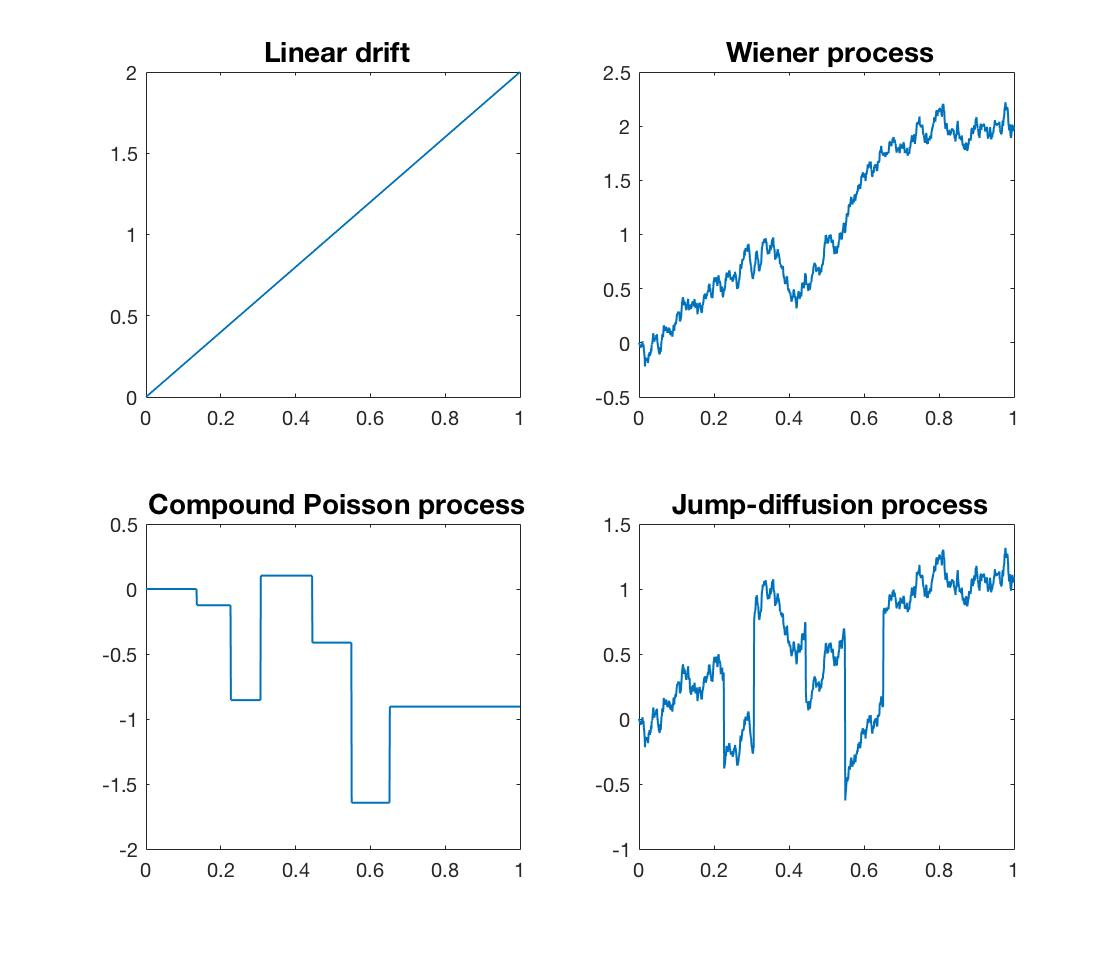
\includegraphics[width=\textwidth]{gfx/processes_examples}
	\caption{Examples of L\'evy processes: a linear drift with L\'evy triplet $(2,0,0)$, a Wiener process with L\'evy triplet $(2,1,0)$, a compound Poisson process with L\'evy triplet $(0,0,\lambda\times f_J)$, where $\lambda = 5$, and $f_J\sim\mathcal{N}(0,1)$ and finally a jump-diffusion process with L\'evy triplet $(2,1,\lambda\times f_J)$.}
	\label{fig:Levy:examples}
\end{figure}

\section{L\'evy measure and path properties}
\label{sec:Levy:Levy_measure}
The \textit{L\'evy measure} dictates the behavior of the jumps.
\begin{defn}[L\'evy measure]
Let $x = \{X_t,t\geq 0\}$ be a L\'evy process on $\mathbb{R}$. The measure $\nu$ on $\mathbb{R}$ defined by
$$\nu(A) = \mathbb{E}\left[\#\{t\in[0,1]:\Delta x \neq 0, \Delta x\in A\}\right],$$
is called the \textbf{L\'evy measure} of $X$: $\nu(A)$ is the expected number, per unit time, of jumps whose size belongs to $A$.
\end{defn}

For example, the L\'evy measure of a compound Poisson process is given by $\nu(dx) = \lambda f_J(dx)$. In other words, the expected number of jumps, in a time interval of length 1, is $\lambda$ and the jump size is distributed according to $f_J$.

More generally, if $\nu$ is a finite measure, that is $\lambda = \nu(\mathbb{R}) =\int_\mathbb{R}\nu(dx) <\infty$, 
then we can defined $f(dx) = \frac{\nu(dx)}{\lambda}$, which is a probability measure. Then, $\lambda$ is the expected number of jumps and $f(dx)$ is the distribution of the jump size $x$. If $\nu(\mathbb{R}) = \infty$, an infinite number of (small) jumps is expected.

\begin{prop}[Finite and infinite activity]
Let $X =\{X_t,t\geq 0\}$ be a L\'evy process with triplet $(\mu,\sigma,\nu)$.
\begin{my_list}
\item If $\nu(\mathbb{R})<\infty$ then almost all paths of $X$ have a finite number of jumps on every compact interval. In that case, the L\'evy process has \textbf{finite activity}.
\item If $\nu(\mathbb{R})=\infty$ then almost all paths of $X$ have a infinite number of jumps on every compact interval. In that case, the L\'evy process has \textbf{infinite activity}.
\end{my_list}
(See Theorem 21.3 in \citeauthor{Sat99} \citeyearpar{Sat99} for the proof)
\end{prop}

Then the L\'evy jump models can be classified into two categories from their L\'evy measure: jump-diffusion or pure jump models. The jump-diffusions models are modeled by a Gaussian part (Wiener process) combined with a jump part (compound Poisson process), that has finitely many jumps in every time interval, i.e. finite activity models. The second category consists of models with an infinite number of jumps in every interval, i.e. infinite activity models. In these models, there is no need of Gaussian part because the dynamics of jumps are already rich enough to generate nontrivial small time behavior. Merton model and Variance Gamma model are respectively good examples of jump-diffusion and pure jump models. We can see in figure \ref{fig:Levy:densities} that the L\'evy density in Variance Gamma model allows infinite number of jumps, while the Merton model has a finite number of jumps on every time interval.

\begin{figure}[!htb]
	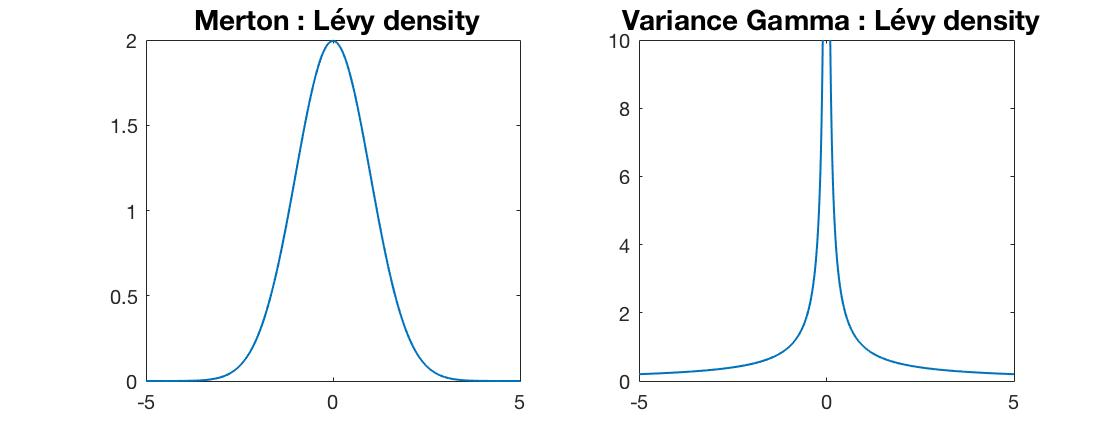
\includegraphics[width=\textwidth]{gfx/Levy_densities}
	\caption{The density of L\'evy measure in the Merton model (left) and the Variance Gamma model (right).}
	\label{fig:Levy:densities}
\end{figure}

\section{Exponential L\'evy processes}
\label{sec:Levy:exponential_processes}

In finance, it is common to model the stock price process as exponentials of a L\'evy process:
$$S_t = S_0 e^{X_t}. $$
The advantage of this representation is that the log returns $\log(S_{t+s}/S_t)$, for $s,t>0,$ follow the distribution of increments of length $s$ dictate by the L\'evy process $X=\{X_t,t\geq0\}$. Thus they have independent and stationary increments. If we choose $X_0=0$, we get $e^{X_0}=1$ and therefore $S_0=S_0e^{X_0}=S_0$. 

In order to avoid an arbitrage opportunity, the discounted stock price process $\hat{S}=\{\hat{S}_t = e^{-rt}S_t,t\geq0\}$ has to be a martingale under an equivalent martingale measure $\mathbb{Q}$, called the \textit{risk neutral measure}. In other words, we are looking for a measure $\mathbb{Q}$ such that
$$\mathbb{E}^\mathbb{Q}\left[\hat{S}_T|\mathcal{F}_t\right]=\hat{S_t}.$$
A first approach is proposed by \citeauthor{Ger94} \citeyearpar{Ger94} using the Esscher transform. This method is a bit complicated and doesn't seem corresponding to the measure chosen by the market. See \citeauthor{Sch03} \citeyearpar{Sch03} for more details.

A second approach consists to correct the mean of the exponential L\'evy process to obtain an equivalent martingale measure $\mathbb{Q}$. This measure is known as the \textit{mean-correcting martingale measure}. The idea behind this method is to change the drift (or add a drift if there is no drift in the process) so that the discounted stock price $\hat{S} = \{\hat{S}_t=e^{-rt}S_t, t\geq 0\}$ becomes a martingale.


% In the case of  a jump-diffusion model, we have
% $$S_t = S_0\exp\left(\mu t+\sigma W_t + \sum_{i=1}^{N_t}Y_i\right)=S_0\exp\left(\mu t+\sigma W_t + J_t\right),$$
% where $J_t$ is the compound Poisson process that dictates the jumps.

% Intuitively, between the jumps, the process evolves like a geometric Brownian motion (Black-Scholes model), and after each jump, $S_t$ is multiplied by the factor $e^{Y_i}$. Thus we can see it as a generalization of the Black-Scholes model:
% $$\frac{dS_t}{S_{t^-}}=\tilde{\mu} dt + \sigma dW_t + dJ_t.$$
% The notation $S_{t^-}$ is used to say that whenever there is a jump, we have to take the value just before the jump in the formula.

\chapter{Numerical Methods}
\label{sec:methods}

\cleanchapterquote{FFT is the most important numerical algorithm of our lifetime.}{Gilbert Strang}{(1934)}

Several methods can be used to price an option under L\'evy process. A method easy to implement and available for exotic options it the \textit{Monte Carlo method}. In this method, we need to simulate a multitude of risk-neutral paths, and then discount the average value of all scenarios. However, this method is very expensive computationally, in particular for a large number of fixing date that forces us to discretize more the paths. The section \ref{sec:methods:MC} is dedicated to this method.

A second way to price exotic options, is to derive the partial differential equation (PDE) or the partial integro differential equation (PIDE) in the case of jump processes. Then we can solve these PDE or PIDE with \textit{Finite Difference method}, for example, to get the price of the option. This method invokes the L\'evy density measure $\nu(dx)$ and could be very complex to implement. We will see that in section \ref{sec:methods:FD}.

A third method, very useful since the density function is often not known in closed form, invokes the characteristic function of the L\'evy process which is always in closed form for L\'evy processes. Then we can use Fourier transform to price the option. Therefore, we will use in section \ref{sec:methods:conv} a method based on Fast Fourier Transform (FFT), which is called the \textit{Convolution method}. This method is very well performing and can be efficiently computed using fast algorithm. 

Finally, we will closed this chapter by summarizing the whole algorithm used to price the FX-TARN.

\section{Monte Carlo Method }
\label{sec:methods:MC}
In this section we will briefly recall the principle of the Monte Carlo simulations and present algorithms to simulate the different processes that we have studied in the last chapter. The idea in the Monte Carlo method is to simulate $M$ sample paths of the stock price process $\mathbf{S}_m, m=1,\ldots,M$, under the corresponding model and, for each path, compute the present value $P(\mathbf{S}_i)$ of the financial product. Then, by the law of the large numbers, we obtain the following proxy:
$$\hat{P}(\mathbf{S})=\frac{1}{M}\sum_{m=1}^M P(\mathbf{S}_m)\xrightarrow{M\to\infty} P(\mathbf{S}),$$
where $\mathbf{S}=(S(t_1),\ldots,S(t_N))$ is the realization of the stock price. The standard error of the estimate is given by
$$\text{SE} = \sqrt{\frac{1}{M-1}\sum_{i=1}^M \left(\hat{P}(\mathbf{S})-P(\mathbf{S}_i)\right)^2}.$$
Remark that the standard error decreases with the square root of the number of sample paths $M$. By the central limit theorem, we can construct the following $95\%$ confidence interval for the real price $P(\mathbf{S})$
$$\left[\hat{P}(\mathbf{S})-1.96\frac{\text{SE}}{\sqrt{M}},\hat{P}(\mathbf{S})+1.96\frac{\text{SE}}{\sqrt{M}} \right]$$

Recall that in our case, the present value of the FX TARN is given by equation \eqref{eq:intro:pv}:
$$P(\mathbf{S}) =N_f \times \sum_{n=1}^N\frac{C^\text{pos}(S(t_n),A(t_{n-1}))+C^\text{neg}(S(t_n),A(t_{n-1}))}{B_d(t_0,t_n)}, \qquad A(t_0)=0,$$
where $C_n$ and $C_n^\ast$ are respectively the gain and the loss on the $n^\text{th}$ fixing date given by equations \eqref{eq:TARN:gain} and \eqref{eq:TARN:loss}. The variable $A(t_n)$ models the accumulated positive cash flow until the date $t_n$ and $B_d(t_0,t_n)^{-1}=e^{-r_d(t_n-t_0)}$ is the domestic discounting factor from $t_n$ to $t_0$. In the rest of the thesis, we will consider the present value per unit of notional $(N_f=1)$.

\subsection{Simulations under Black-Scholes model}
We have seen that the L\'evy process in the Black-Scholes model is given by
$$X_t^\text{BS} = \left(r-q-\frac{1}{2}\sigma^2\right)t +\sigma W_t,$$
where $W_t$ is a Wiener process. Therefore, by discretization of time, we get
$$\Delta X_t^\text{BS}=\left(r-q-\frac{1}{2}\sigma^2\right)\Delta t+\sigma \sqrt{\Delta t}Z,$$
with $Z\sim\mathcal{N}(0,1)$. Finally we easily have
\begin{align*}
S_{t+\Delta t} &= \exp\left\{X_t^\text{BS}+\left(r-q-\frac{1}{2}\sigma^2\right)\Delta t+\sigma\sqrt{\Delta t}Z\right\}\\
&= S_t\exp\left\{\left(r-q-\frac{1}{2}\sigma^2\right)\Delta t+\sigma\sqrt{\Delta t}Z\right\}.
\end{align*}
We can use the command \textbf{\texttt{random('norm',0,1)}} in \textsc{Matlab} to generate random normal variable. Figure \ref{fig:MC:BS} shows five simulated sample paths under Black-Scholes model.
\begin{figure}[!htb]
	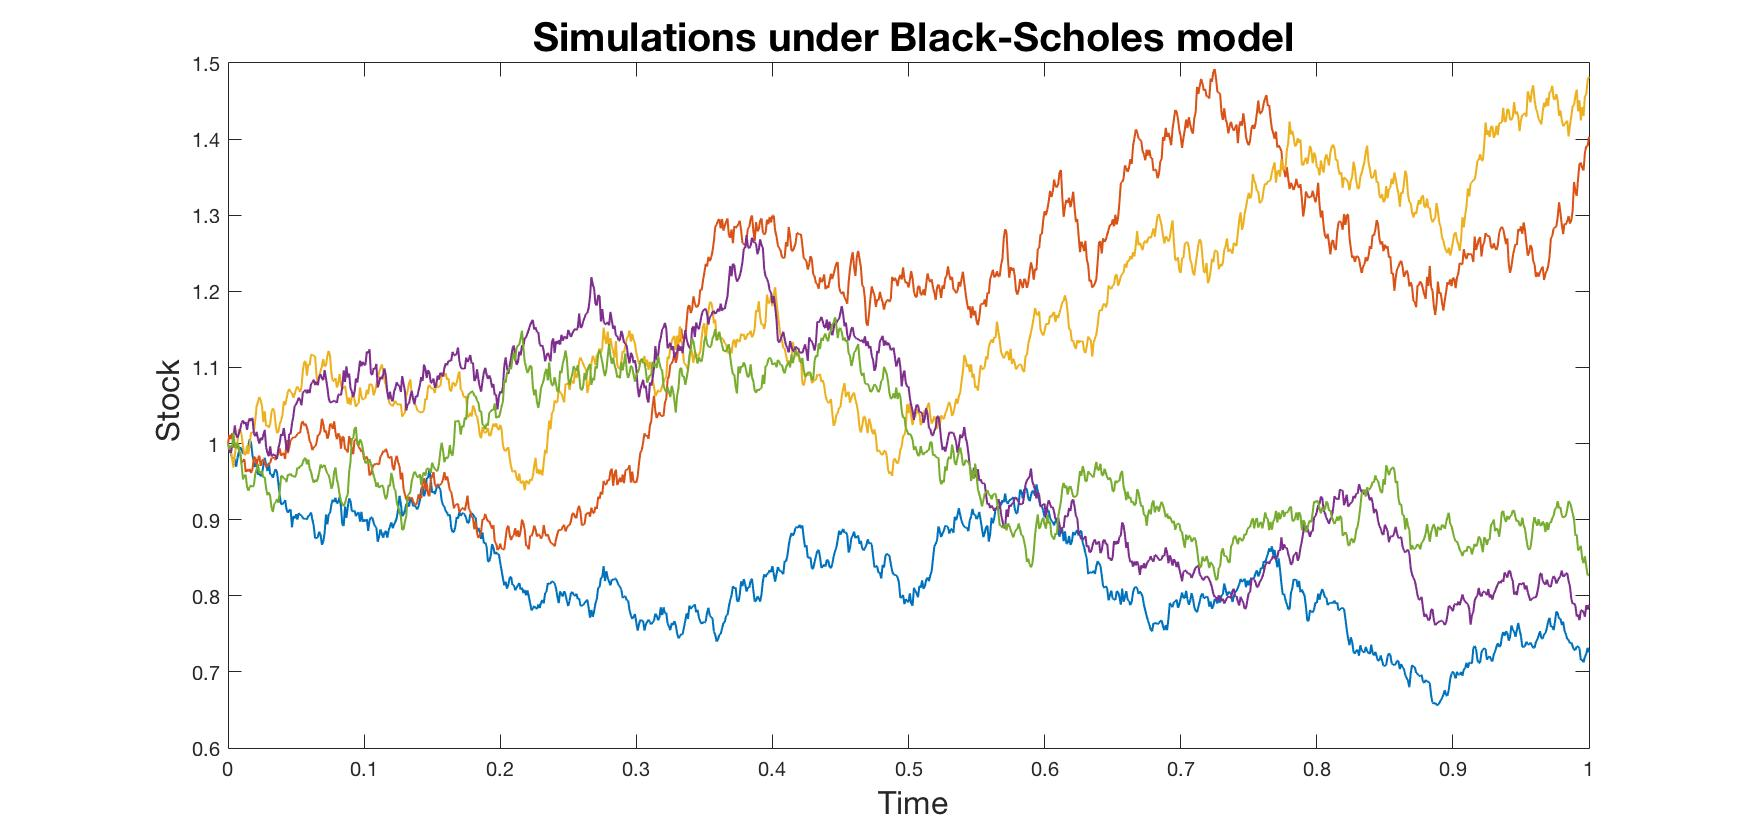
\includegraphics[width=\textwidth]{gfx/BS_plot}
	\caption{Simulations of stock price process under Black-Scholes model.\\ $S_0=1, r= 0.01,q = 0.02, \sigma=0.3, T = 1, dt = 0.001, M=5$.}
	\label{fig:MC:BS}
\end{figure}

\subsection{Simulations under Jump-diffusion models}
A jump-diffusion process is nothing else than a Brownian motion with drift to which a jump process modeled by a compound Poisson process is added. In other words, we have
$$X_t^\text{JD} = \gamma^\ast t + \sigma W_t + \sum_{i=1}^{N_t}Y_i,$$
where $N_t\sim\text{Poisson}(\lambda t)$ and the jump size $Y_i$ has density function $f_J$. We have seen the two special cases where the distribution $f_J$ is normal $\mathcal{N}(\alpha,\delta^2)$ in the Merton model and double exponential $\text{DoubleExp}(p,\eta_1,\eta_2)$ in the Kou model.

Therefore, we have that
$$\Delta X_t^\text{JD} = \gamma^\ast \Delta t + \sigma \sqrt{\Delta t} Z + J(\Delta t),$$
where $J(\Delta t)$ is the sum of all jumps between $t$ and $t+\Delta t$, i.e.
$$J(\Delta t)=\sum_{i=1}^{N_{\Delta t}}Y_i.$$
We can use the command \textsc{Matlab} \texttt{random('poiss',$\lambda \Delta t$)} to simulate the variable $N_{\Delta t}$.
\subsubsection{Merton model}
In his model, \citeauthor{Mer76} supposed that the jump size is normally distributed with mean $\alpha$ and standard deviation $\delta$, i.e. $Y_i\sim\mathcal{N}(\alpha,\delta)$. Then, recall that the risk-neutral drift is given by
$$\gamma^\ast = r-q-\frac{1}{2}\sigma^2-\lambda\left(e^{\alpha+\frac{1}{2}\delta^2}-1\right).$$
Thus we have
$$S_{t+\Delta t} = S_t\exp\left\{\gamma^\ast \Delta t + \sigma \sqrt{\Delta t}Z + J(\Delta t)\right\},$$
where $J(\Delta t)\sim\mathcal{N}(N_{\Delta_t}\alpha,N_{\Delta t}\delta)$ and $N_{\Delta t}\sim\text{Poisson}(\lambda\Delta t)$.

Finally, we obtain the results of five simulated sample paths in figure \ref{fig:MC:Mer}.
\begin{figure}[!htb]
	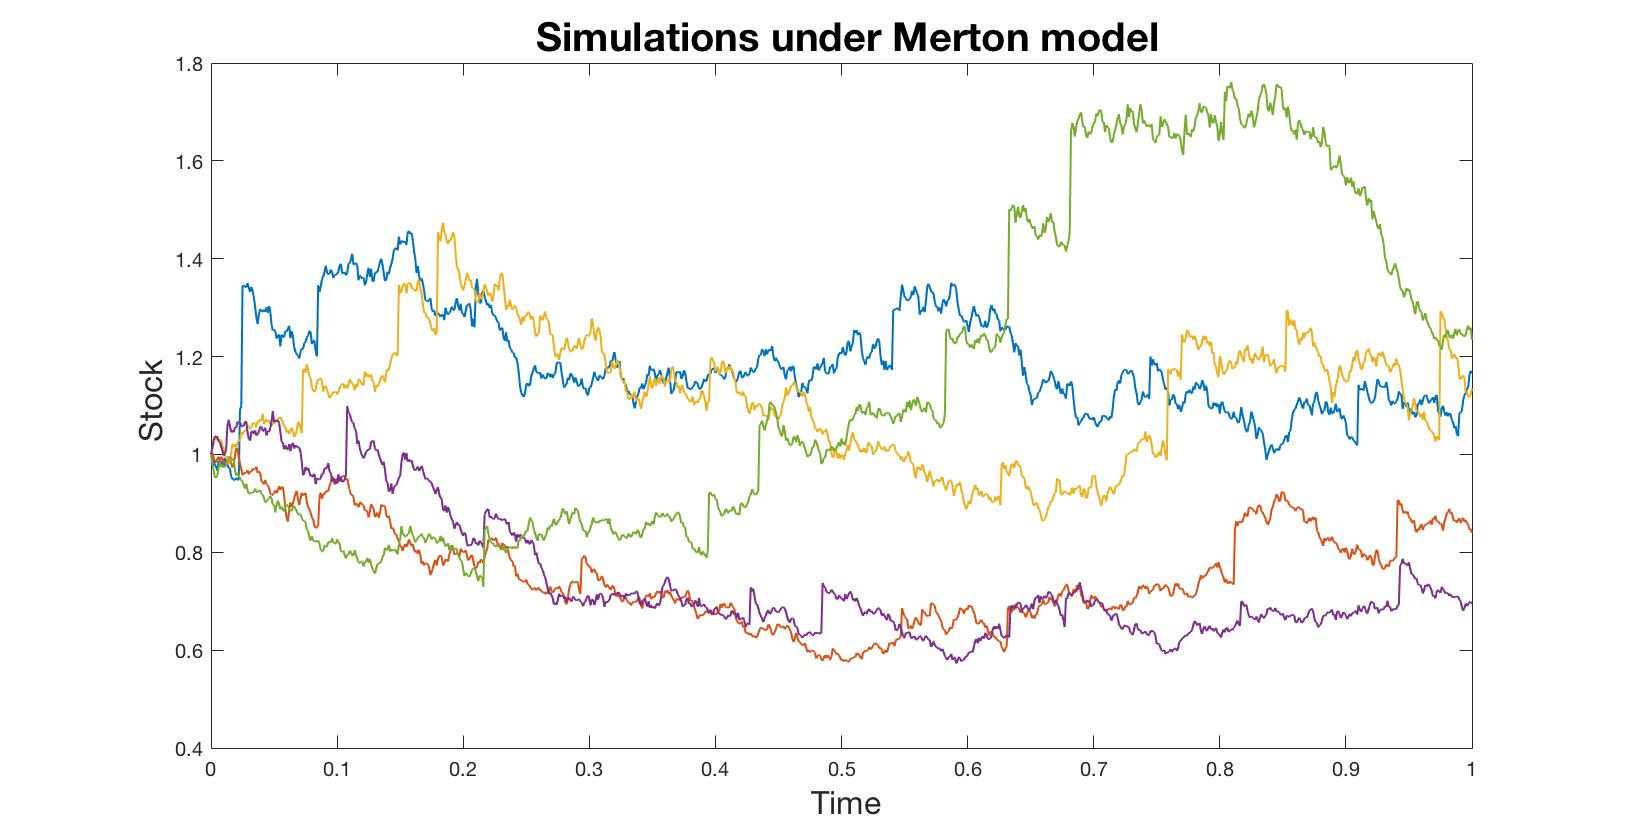
\includegraphics[width=\textwidth]{gfx/Merton_plot}
	\caption{Simulations of stock price process under Merton model.\\ $S_0=1, r= 0.06,q = 0.02,\lambda = 10 , \alpha = 0.1, \delta = 0.05, \sigma=0.3,$\\$T = 1, dt = 0.001, M=5$.}
	\label{fig:MC:Mer}
\end{figure}

\newpage
\subsubsection{Kou model}
This model is very similar to the Merton's one, but \citeauthor{Kou02} proposed to use a double exponential distribution for the jump size, i.e. $Y_i\sim\text{DoubleExp}(p,\eta_1,\eta_2)$. Thus the difficulty is to simulate double exponential random variables. Note that the sum of $K$ independent exponential random variables of parameter $\eta$ has a gamma distribution with parameters $K$ and $\eta$. In other words, if $X_1,\ldots,X_K\sim\text{Exp}(\eta)$, then $Y = \sum_{i=1}^K X_i\sim\Gamma(K,\eta)$ and
$$f_Y(y) = y^{K-1}\frac{\eta^K e^{-\eta y}}{K-1}.$$
Hence, to simulate the jumps $J(\Delta t)$, we begin by simulating a binomial random variable $K$ that counts the number of positive jumps in $[t,t+\Delta t]$,
$$K \sim \text{Binomial}(N_{\Delta t},p), \qquad \text{ with } N_{\Delta t}\sim \text{Poisson}(\lambda\Delta t).$$
Then, we simulate the positive and negative jumps
\begin{align*}
J^+&\sim\text{Gamma}(K,\eta_1), \\
J^-&\sim\text{Gamma}(N_{\Delta t}-K,\eta_2).
\end{align*}
This reads in \textsc{Matlab} as \texttt{random('gam',$K,1/\eta_i$)} because the convention of the parameters (shape/scale versus shape/rate).

Therefore the sum of jumps in the time interval $[t,t+\Delta t]$ is given by
$$J(\Delta t) = J^+-J^-.$$
At the end, we have the same representation of the stock price as before
$$S_{t+\Delta t} = S_t\exp\left\{\gamma^\ast \Delta t + \sigma \sqrt{\Delta t}Z + J(\Delta t)\right\},$$
with
$$ \gamma^\ast=r-q- \frac{1}{2}\sigma^2 -\lambda \left(\frac{p\cdot\eta_1}{\eta_1+1}+\frac{(1-p)\cdot\eta_2}{\eta_2+1}-1\right).$$
The simulation of sample paths under Kou model are illustrated in figure \ref{fig:MC:Kou}
\begin{figure}[!htb]
	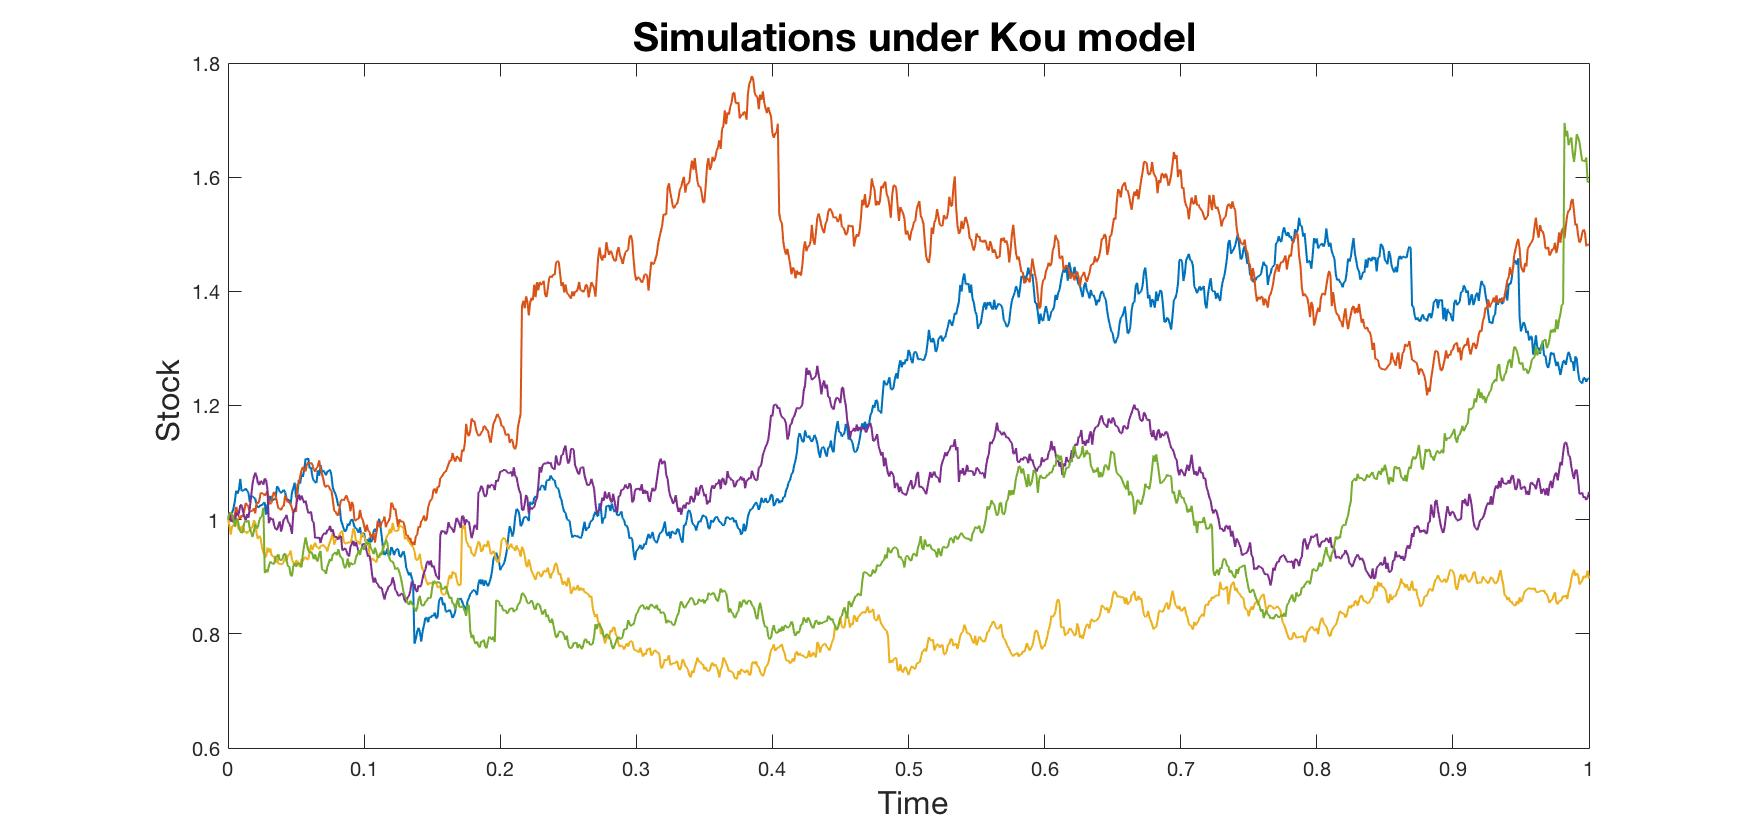
\includegraphics[width=\textwidth]{gfx/Kou_plot}
	\caption{Simulations of stock price process under Kou model.\\ $S_0=1, r= 0.06,q = 0.02,\lambda = 10 , p = 0.55, \eta_1 =\eta_2= 25, \sigma=0.3,$\\$T = 1, dt = 0.001, M=5$.}
	\label{fig:MC:Kou}
\end{figure}

\subsection{Simulations under Pure jump models}
Recall that a pure jump process, as Normal Inverse Gaussian (NIG) process or Variance Gamma (VG) process, can be seen as a Brownian subordination
$$X_t^\text{PJ} = \theta T_t + \sigma W_{T_t},$$
where $T=\left\{T_t,t\geq0\right\}$ is a random time process, called the \textit{subordinator}. The goal is then to simulate this subordinator and substitute it to the time of a Brownian motion with drift. In the Normal Inverse Gaussian model, this time subordinator will be an Inverse Gaussian process, and in the Variance Gamma model, it will be a Gamma process.

\subsubsection{Normal Inverse Gaussian model}
First of all, recall that the L\'evy process in the Normal Inverse Gaussian model is given by
$$X_t^\text{PJ} = \beta \delta^2 T_t + \delta W_{T_t},$$
with $T_t\sim \text{IG}\left(t,\delta \sqrt{\alpha^2-\beta^2}\right)$.
Hence we have to construct a Normal Inverse Gaussian (NIG) process. To do that, we simulate an Inverse Gaussian (IG) process and set it as time parameter of the Brownian motion. In fact, we have that
$$\Delta X_t^\text{PJ} = \beta\delta^2\Delta T_t+\delta \sqrt{\Delta T_t}Z, $$
where $\Delta T_t\sim\text{IG}\left(\Delta t, \delta \sqrt{\alpha^2-\beta^2}\right)$ and $Z\sim\mathcal{N}(0,1)$.

Finally, we have the stock price sample path
$$S_{t+\Delta t}=S_t\exp\left\{\gamma^\ast\Delta t + \Delta X_t^\text{PJ}\right\},$$
with $\gamma^\ast=r-q -\delta \left(\sqrt{\alpha^2-\beta^2}-\sqrt{\alpha^2-(\beta+1)^2}\right)$.
Be careful with the convention of the \textsc{Matlab} command \texttt{random('inversegaussian',$\mu,\lambda$)}, where $\mu = \frac{a}{b}$ is the mean and $\lambda = a^2$ is the shape parameter. We can see the result of five sample path in figure \ref{fig:MC:NIG}.
\begin{figure}[!htb]
	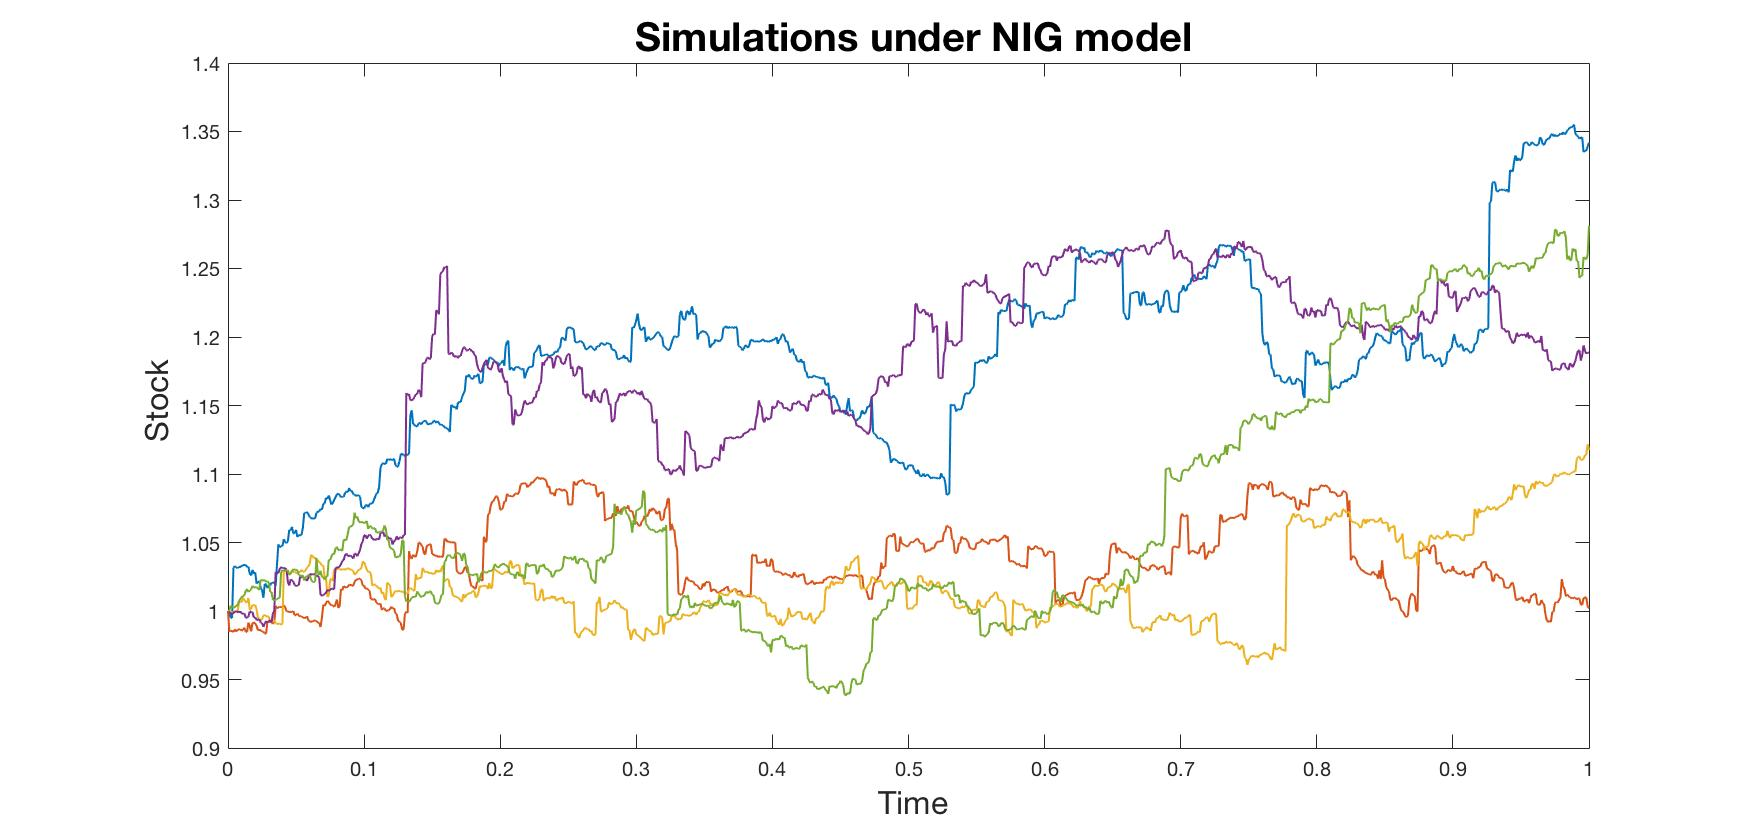
\includegraphics[width=\textwidth]{gfx/NIG_plot}
	\caption{Simulations of a stock price process under NIG model.\\ $S_0=1, r= 0.06,q = 0.02,\alpha = 50 , \beta = 3, \delta = 1,$\\$T = 1, dt = 0.001, M=5$.}
	\label{fig:MC:NIG}
\end{figure}
\subsubsection{Variance Gamma model}
Following the same procedure as before, we just have to change the time subordinator process by taking a Gamma process. Then we have the time-changed Brownian motion
$$X_t^\text{PJ}=\theta T_t + \sigma W_{T_t},$$
with $T_t\sim \text{Gamma}\left(\frac{t}{\nu},\frac{1}{\nu} \right)$. Therefore, we get
$$\Delta X_t^\text{PJ} = \theta \Delta T_t + \sigma \sqrt{\Delta T_t} Z,$$
where $\Delta T_t\sim\text{Gamma}\left(\frac{\Delta t}{\nu},\frac{1}{\nu}\right)$ and $Z\sim\mathcal{N}(0,1)$.
Thus we get
$$S_{t+\Delta t} = S_t \exp\left\{\gamma^\ast\Delta t + \Delta X_t^\text{PJ}\right\},$$
with $\gamma^\ast = r-q + \frac{1}{\nu}\ln\left(1-\theta\nu-\frac{\sigma^2\nu}{2}\right)$.
The figure \ref{fig:MC:VG} illustrates the result of five simulations under this last model.
\begin{figure}[!htb]
	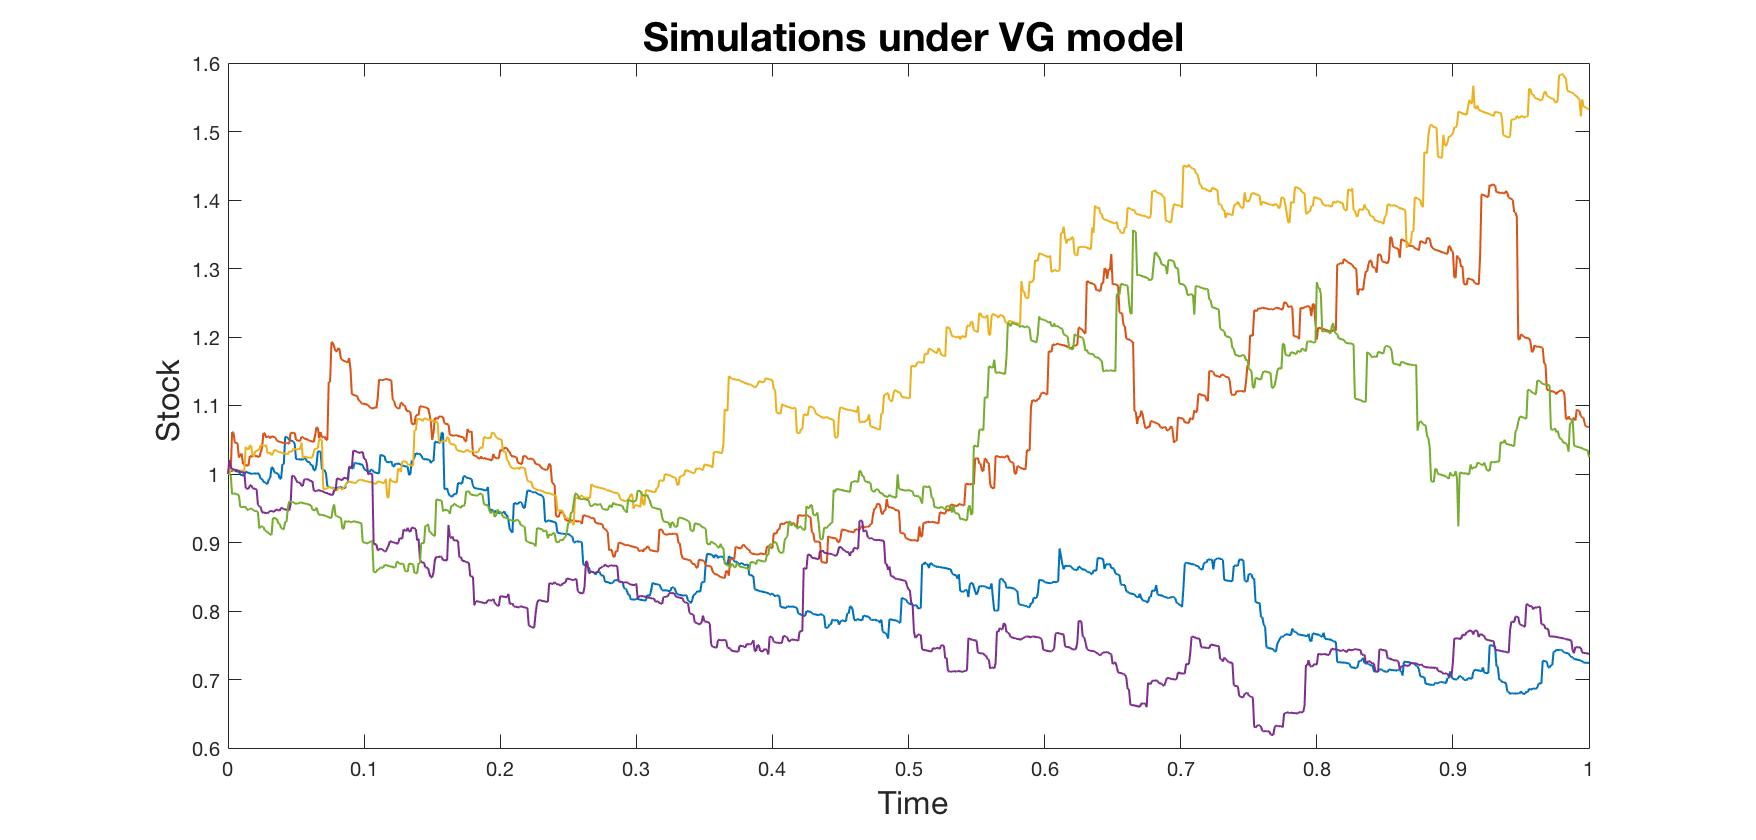
\includegraphics[width=\textwidth]{gfx/VG_plot}
	\caption{Simulations of a stock price process under VG model.\\ $S_0=1, r= 0.06,q = 0.02,\theta = 0.5 , \sigma = 0.3, \nu = 0.01,$\\$T = 1, dt = 0.001, M=5$.}
	\label{fig:MC:VG}
\end{figure}

\subsection{Pricing FX-TARN with Monte Carlo}
Note that for the pricing of the FX TARN it suffices to take $\Delta t$ equal to the difference of two consecutive fixing dates, i.e. the length of a period (e.g. Daily/Weekly/Monthly). It is not necessary to simulate the points between these dates because the cash flows depend only on the observations on the fixing dates.

From the simulations above, and equations \eqref{eq:TARN:gain} and \eqref{eq:TARN:loss}, this is easy to compute the payoff on each fixing dates $t_n, (n=1,\ldots,N)$, with respect to the realization $S_{t_n}$. This is also necessary to update the variable $A(t_n)$ that takes into account the accumulated gain. 

Finally, we have for each simulated scenario $\mathbf{S}_m, (m=1,\ldots,M)$, the present value from equation \eqref{eq:intro:pv}
$$P(\mathbf{S}_m) = \sum_{n=1}^{N}e^{-r_d t_n}C^\text{tot}(S(t_n),A(t_{n-1})),$$
where we have taken $B_d(t_0,t_n)^{-1}=e^{-r_d (t_n-t_0)}$, with $r_d$ the domestic risk-free rate. Hence, the value of the FX-TARN obtained with the Monte-Carlo method is given by
$$\hat{P}(\mathbf{S})=\frac{1}{M}\sum_{m=1}^M P(\mathbf{S}_m).$$

\section{Finite Difference Method}
\label{sec:methods:FD}
This section is devoted to the Finite Difference (FD) method for different models. We will see how to solve numerically the PDE in Black-Scholes model and the PIDE in the jump-diffusion and pure jump models. The central tool of L\'evy processes in FD method is the L\'evy measure $\nu$ used to characterize the jumps in the integral part of the PIDE. In the case of Black-Scholes, we have seen that this measure is null.

\subsection{Black-Scholes world}
A Finite Difference method to price Target Accrual Redemption Note (TARN) under (generalized) Black-Scholes model was proposed by \citeauthor{LS15} \citeyearpar{LS15} \cite{LS15}. To summarize, their approach, consider the value of the FX-TARN $V(S,t,A)$, where $S$ is the spot rate and $A$ is the accumulated amount until time $t$. Since the accumulation $A$ has no effect in the diffusion between two fixing dates, the Black-Scholes option pricing PDE is still valid
\begin{equation}\label{eq:PDE}
\frac{\partial V}{\partial t}+\frac{1}{2}\sigma^2(S,t)S^2\frac{\partial^2 V}{\partial S^2}+\left(r_d(t) -r_f(t)\right)S\frac{\partial V}{\partial S}-r_d(t) V = 0,
\end{equation}
with $r_d$ and $r_f$ respectively the domestic and foreign risk free rates.

At the end of the product's life, there is no more coming cash flow. Therefore at time $T$, the value of the option is null. Hence we can consider the terminal condition to be
$$V(S,T,A) = 0.$$
However, just before the  last fixing date, at $T^-=t_N^-$, the value is equal to the last payment 
$$V(S,t_N^-,A(t_N^-)) = C^\text{pos}(S,A(t_{N-1})) + C^\text{neg}(S,A(t_{N-1})=\mathbf{C}^\text{tot}_N(S,A(t_{N-1})),$$
where $C^\text{pos}$ and $C^\text{neg}$ are respectively the positive and the negative cash flows at time $t_N$, given by equations \eqref{eq:TARN:gain} and \eqref{eq:TARN:loss}, and $\mathbf{C}^\text{tot}_N$ is the total cash flow. Note that the accumulated amount $A$ is a discontinuous piecewise constant process. Moreover, this is a cadlag process. Then we have that $A(t_n^-) = A(t_{n-1})$ and $A(t_n^+) = A(t_n)$ for $n = 1,\ldots,N$.

The total cash flow on the $n$\textsuperscript{th} fixing date $t_n$ makes a jump in the value of the product. In other words, at $t_n^-$, the value is given by
\begin{align}\label{eq:jump_cond}
V(S,t_n^-,A(t_n^-)) &= V(S,t_n,A(t_n))+C^\text{tot}(S,A(t_{n-1}))\nonumber\\
&=V(S,t_n,A(t_{n-1})+C^\text{pos}(S,A(t_{n-1})))+C^\text{tot}_n(S,A(t_{n-1})).
\end{align}

Finally, we can get the today's FX-TARN price by taking $ V_0 = V(S(t_0),t_0,0)$.

\subsubsection{Finite difference scheme and Cubic spline interpolation}
First of all, consider the time interval between two successive fixing dates $[t_n,t_{n+1}]$ on which the diffusion by Finite Difference method is done. An uniform discretization gives us the time grid $t_k = t_n + k\Delta t, k = 0,1,\ldots,N_t$. Then a discretization in the spot price variable $S$ is given by a grid $0<S_{\min}=S_1<\cdots<S_M=S_{\max}$.

In order to get this final solution, the idea of \citeauthor{LS15} is to introduce an auxiliary finite grid $0 = A_1<A_2<\cdots<A_{N_a}= U$ to track the accumulated amount, where $U$ denotes the target. Then the goal is to perform $N_a$ finite difference solutions between all fixing dates, for each value $A_j$ of accumulated amount, which correspond to a different "scenario". 

For the fixing date $t_{n+1}$, if we associate the node $A_j$ to the accumulated amount $A(t_{n})$, the equation \eqref{eq:jump_cond} can be written as
$$V(S_m,t^-_{n+1},A_j) = V(S_m,t_{n+1},A^+_j)+ C^\text{tot}(S_m,A_j),$$
with $A_j^+ = A_j + C^\text{pos}(S_m,A_j)$, for $m=1,\ldots,M$. This quantity is used as initial condition at the beginning of each finite difference scheme.

Since only the value $V(S_m,t_{n+1},A_j)$ is known after a diffusion step, we have to evaluate $V(S_m,t_{n+1},A_j^+)$ by cubic spline interpolation. Hence for a fixed $j$, we can extract $N_a$ values $V(S_m,t_{n+1},A_j^+)$ by interpolating $V(S_m,t_{n+1},A_j)$ with respect to $A_j$.

To perform the finite difference step, it is common to write equation \eqref{eq:PDE} in terms of log asset price $x = \log(S)$ and time to maturity $\tau=T-t$. However, here we do not consider the Finite Different scheme until the maturity $T$. Then we will use $\tau = t_{n+1}-t$ for $t\in(t_n,t_{n+1})$. This gives us the following PDE
$$\frac{\partial V}{\partial \tau}-\frac{1}{2}\sigma^2\frac{\partial^2 V}{\partial x^2}-\left(r_d - r_f - \frac{1}{2}\sigma^2\right)\frac{\partial V}{\partial x}+r_d V = 0.$$
The advantage of this representation is that in a Black-Scholes world with constant parameters, all the coefficient are constant. Therefore the finite difference grid in $x$ is given by $\log(S_{\min}) = x_0 < x_1<\cdots<x_M = \log(S_{\max})$. 

Let us denote the option price at time $\tau_k = t_{n+1}-t_k$, and grid point $x_i$ as $V_i^k$, for $k=0,1,\ldots, N_t$. Hence, for an uniform grid, $\Delta x_i = x_i-x_{i-1} = \Delta x$, we get the finite difference approximation with second order accuracy 
\begin{align*}
\frac{\partial V}{\partial x}(x_i,\tau_k,A_j) &= \mathcal{D}_{\Delta x} V +\mathcal{O}(\Delta x^2),\\
\frac{\partial^2 V}{\partial x^2}(x_i,\tau_n) &= \mathcal{D}_{\Delta x}^2 V+\mathcal{O}(\Delta x^2),
\end{align*}
where 
\begin{align*}
\mathcal{D}_{\Delta x} V&= \frac{V_{i+1}^k-V_{i-1}^k}{2\Delta x},\\
\mathcal{D}^2_{\Delta x}V &= \frac{V_{i+1}^k-2V_i^k+V_{i-1}^k}{\Delta x^2}.
\end{align*}

Then with the finite difference operator $F_i^n$ defined as
$$F_i^k \equiv -\frac{1}{2}\sigma^2\mathcal{D}_{\Delta x}^2V-\left(r_d - r_f - \frac{1}{2}\sigma^2\right)\mathcal{D}_{\Delta x}V+r_d V,$$
the $\theta$-scheme can be expressed as
$$\frac{V_i^{n+1}-V_i^n}{\Delta t}+\theta F_i^{n+1} +(1-\theta)F_i^n=0,\qquad \begin{cases}i = 1,\ldots, M-1\\k = 0,\ldots,N_t-1 \end{cases}$$
with $\theta\in[0,1]$. The special cases $\theta=0,\theta=0.5$ and $\theta=1$ correspond respectively to the fully explicit, Crank-Nicholson and fully implicit scheme.

\subsubsection{Boundary Conditions}
Recall that the fixing dates in time to maturity notation can be written as
\begin{align*}
\tau_0 &= T-t_N = 0,\\
\tau_1 &= T-t_{N-1},\\ 
&\quad\vdots\\ 
\tau_N &= T-t_0 = T.
\end{align*}

Hence, for $\tau \in (\tau_0,\tau_1)$, the value of the product depends only on the last expected cash flow. Therefore, the Dirichlet boundary conditions are given by
\begin{align*}
V(x_{\max},\tau,A) &= C^\text{tot}\left(e^{x_{\max}+(r_d-r_f)\tau},A\right)e^{-r_d\tau}\\
&= \left(C^\text{pos}\left(e^{x_{\max}+(r_d-r_f)\tau},A\right)+C^\text{neg}\left(e^{x_{\max}+(r_d-r_f)\tau},A\right)\right)e^{-r_d\tau},
\end{align*}
and
\begin{align*}
V(x_{\min},\tau,A) &= C^\text{tot}(e^{x_{\min}+(r_d-r_f)\tau},A)e^{-r_d\tau}\\
&= \left(C^\text{pos}\left(e^{x_{\min}+(r_d-r_f)\tau},A\right)+C^\text{neg}\left(e^{x_{\min}+(r_d-r_f)\tau},A\right)\right)e^{-r_d\tau}.
\end{align*}

For $\tau \in (\tau_n,\tau_{n+1}), n= 1,\ldots,N-1$, the expected value at maturity depends only on the next positive cash flow, since then the product knocks out after a large gain, and on all coming negative cash flows, since there is no decumulation in the accumulation variable $A$ due to a loss. Thus the boundary condition are this time
\begin{align*}
V(x_{\max},\tau,A) &= C^\text{pos}\left(e^{x_{\max}+(r_d-r_f)(\tau-\tau_n)},A\right)e^{-r_d(\tau-\tau_n)}\\
&\quad + \sum_{j = 0}^n C^\text{neg}\left(e^{x_{\max}+(r_d-r_f)(\tau-\tau_j)},A\right)e^{-r_d(\tau-\tau_j)},
\end{align*}
and
\begin{align*}
V(x_{\min},\tau,A) &= C^\text{pos}\left(e^{x_{\min}+(r_d-r_f)(\tau-\tau_n)},A\right)e^{-r_d(\tau-\tau_n)}\\
&\quad + \sum_{j = 0}^n C^\text{neg}\left(e^{x_{\min}+(r_d-r_f)(\tau-\tau_j)},A\right)e^{-r_d(\tau-\tau_j)}.
\end{align*}

Note that we do not have to discount the cash flows until maturity, because they are made on the fixing dates.

\subsection{Jump-diffusion models}
To go beyond the Black-Scholes world, we can generalize this method to the jump-diffusion models. As proposed by \citeauthor{CV05} \citeyearpar{CV05} \cite{CV05}, we can solve numerical the Partial Integro Differential equation (PIDE) evolving under L\'evy processes. The PIDE is given by
\begin{align*}\frac{\partial V}{\partial \tau}&-\frac{1}{2}\sigma^2\frac{\partial^2V}{\partial x^2}-\left(r_d-r_f-\frac{1}{2}\sigma^2\right)\frac{\partial V}{\partial x}+r_d V \\
&-\int_{-\infty}^\infty \left[V(x+y,\tau,A)-V(x,\tau,A)-\left(e^y-1\right)\frac{\partial V}{\partial x}(x,\tau,A)\right]\nu(dy) = 0,
\end{align*}
where $\nu(\cdot)$ is the L\'evy measure of the process $X =\{X_t,t\geq0\}$ that characterizes the log asset price. Recall that in the Merton and Kou models, the L\'evy density is, respectively, given by
\begin{align*}
\nu^\text{Mer}(dy) &= \frac{\lambda}{\sqrt{2\pi}\delta}e^{-\frac{(y-\alpha)^2}{2\delta^2}}dy,\\
\nu^\text{Kou}(dy) &= \lambda\left(p\cdot\eta_1e^{-\eta_1 y} \mathbf{1}_{y\geq0}+(1-p)\cdot\eta_2e^{\eta_2y}\mathbf{1}_{y<0}\right)dy.
\end{align*}

Therefore, some integral terms can be analytically computed as
\begin{align*}
\int_{-\infty}^\infty \nu^\ast(dy) &= \lambda, \qquad \text{with } \nu^\ast = \nu^\text{Mer} \text{ or } \nu^\text{Kou},\\
\int_{-\infty}^\infty (e^y-1)\nu^\text{Mer}(dy) &= \lambda\left(e^{\alpha +\frac{1}{2}\delta^2}-1\right)\equiv c,\\
\int_{-\infty}^\infty (e^y-1)\nu^\text{Kou}(dy) &= \lambda\left(\frac{p\eta_1}{\eta_1-1}+\frac{(1-p)\eta_2}{\eta_2+1}-1\right)\equiv c.
\end{align*}

Hence, we can rewrite the PIDE in the form
\begin{align*}\frac{\partial V}{\partial \tau}-\frac{1}{2}\sigma^2\frac{\partial^2V}{\partial x^2}&-\left(r_d-r_f-\frac{1}{2}\sigma^2 -c\right)\frac{\partial V}{\partial x}+(r_d +\lambda)V \\
&-\int_{-\infty}^\infty V(x+y,\tau,A)\nu(dy) = 0,
\end{align*}

Note that in the log asset price form, the last integral term $\int_{-\infty}^\infty V(x+y,\tau,A)\nu(dy)$ has a convolution structure that allows us to compute it by Fast Fourier Transform (FFT). This is not the case in the asset price PIDE.

\subsubsection{Localization to a bounded domain}
To solve this numerical problem, we first truncate the space domain to a bounded interval $x\in(x_{\min},x_{\max})$ as usually. The boundary conditions are the same as in the Black-Scholes case. Hence the truncated Cauchy problem reads
$$\begin{cases}
\displaystyle{\frac{\partial V}{\partial \tau}-\frac{1}{2}\sigma^2\frac{\partial^2V}{\partial x^2}-\left(r_d-r_f-\frac{1}{2}\sigma^2-c\right)\frac{\partial V}{\partial x}+(r_d+\lambda) V} \\
\hspace{3cm}\displaystyle{-\int_{-\infty}^\infty V(x+y,\tau,A)\nu(dy) = 0}, \hspace{2cm}x\in(x_{\min},x_{\max}),\\
V(x,\tau,A) = \Psi(x,\tau,A), \hspace{6.3cm} x \not\in (x_{\min},x_{\max}),
\end{cases}$$
where $$ \Psi(x,\tau,A) = .$$
Observe that the integral term $\int_{-\infty}^\infty V(x+y,\tau)\nu(dy)$ still involves the values of $V(x,t,A)$ outside of the truncated domain. Hence the boundary conditions have to be imposed for all $x\not\in(x_{\min},x_{\max})$ and not only at the two boundary points $x_{\min}$ and $x_{\max}$.

\subsubsection{Truncation of the integral}
For computational purpose, we need to truncate the integral term,
$$J = \int_{-\infty}^\infty V(x+y,\tau)\nu(dy),$$
as
$$J_{B_l,B_r} = \int_{-B_l}^{B_r} V(x+y,\tau,A)\nu(dy).$$
In practice, it is more convenient to use a variable truncation on $$[-(x-x_{\min})-B_l, (x_{\max}-x)+B_r] \supset [-B_l,B_r].$$
Therefore, we get
$$J\approx \int_{-(x-x_{\min})-B_l}^{(x_{\max}-x)+B_r} V(x+y,\tau,A)\nu(dy).$$
If the L\'evy measure $\nu$ has density $\nu(dy) = k(y) dy$, which is the case in Merton or Kou model, we have 
$$J\approx \int_{x_{\min}-B_l}^{x_{\max}+B_r} V(z,\tau,A)k(z-x)dz.$$
Hence, the fully truncated problem can be written as
$$\begin{cases}
\displaystyle{\frac{\partial V}{\partial \tau}-\frac{1}{2}\sigma^2\frac{\partial^2V}{\partial x^2}-\left(r_d-r_f-\frac{1}{2}\sigma^2-c\right)\frac{\partial V}{\partial x}+(r_d + \lambda) V} \\
\hspace{3cm}\displaystyle{-\int_{x_{\min}-B_l}^{x_{\max}+B_r} V(z,\tau,A)k(z-x)dz = 0}, \hspace{1cm} x\in(x_{\min},x_{\max}),\\
V(x,\tau,A) = \Psi(x,\tau,A), \hspace{2.3cm} x \in [x_{\min}-B_l,x_{\min}]\cup[x_{\max},x_{\max}+B_r].
\end{cases}$$

\subsubsection{Finite difference approximation}
The major change from the simple case of a PDE is to extend the spatial grid to be able to compute the integral part outer of the original grid. In other words, consider the following original and extended spatial grid
\begin{align*}
x_i &= x_{\min}+ i\Delta x, \qquad\text{for } i \in I = \{1,M-1\},\\
x_i &= x_{\min}+i\Delta x, \qquad\text{for } i \in \tilde{I}=\{-K_l, \ldots, M + K_r\}.
\end{align*}
One way to compute the integral term is to use the trapezoidal rule using the extended computational grid $j\in \tilde{I}$. This means that for a continuous function $f:\mathbb{R}\to\mathbb{R}$ and an internal grid point $x_i$, denoting $k_i= k(x_i)$, we have
$$\int_{x_{\min}-B_l}^{x_{\max}+B_r} f(z) k(z-x_i) \approx \sum_{l=-K_l}^{M+K_r}\Delta x f(x_l)k(\underbrace{x_l-x_i}_{x_{l-i}})=\sum_{-K_l}^{M+K_r}\Delta x f(x_l)k_{l-i}.$$
Hence our integral can be approximated by
$$\int_{x_{\min}-B_l}^{x_{\max}+B_r} V(z,\tau_n)k(z-x)dz\approx \Delta x \sum_{l=-K_l}^{M+K_r} V^n_l k_{l-i}.$$
This development brings us to the \textit{Forward Euler} finite difference approximation
$$\begin{cases}
\displaystyle{\frac{V_i^{k+1}-V_i^k}{\Delta t}-\frac{1}{2}\sigma^2\frac{V_{i+1}^k-2V_i^k+V_{i-1}^k}{\Delta x^2}-\left(r_d-r_f-\frac{1}{2}\sigma^2-c\right)\frac{V_{i+1}^k-V_{i-1}^k}{2\Delta x}} \\
\hspace{3cm}\displaystyle{+(r_d + \lambda) V_i^k
-\Delta x \sum_{l=-K_l}^{M+K_r}V_l^k k_{l-i} = 0}, \hspace{1cm} i \in I,\\
V_i^k = \Psi(x_i,\tau_k,A), \hspace{7cm} i\in\tilde{I}\backslash I.
\end{cases}$$

With the following vectorial notation 
\begin{align*}
\mathbf{V}^k = \{V_i^k, i \in I\} & \text{: vector of unknowns on internal nodes},\\
\mathbf{\tilde{V}}^k = \{V_i^k, i \in \tilde{I}\}& \text{: vector of nodal values on the extended grid},
\end{align*}
we can write the Forward Euler finite difference in the algebraic form as
$$\begin{cases}
\displaystyle{\frac{\mathbf{V}^{k+1}-\mathbf{V}^k}{\Delta t}+ A\mathbf{V}^k-J\mathbf{\tilde{V}}^k = \mathbf{F}^k},&k = 0,\ldots, N_t-1,\\
\mathbf{\tilde{V}}_I^{k+1} = \mathbf{V}^{k+1},\qquad \mathbf{\tilde{V}}_{\tilde{I}\backslash I}^{k+1}=\mathbf{\Psi}_{\tilde{I}\backslash I}^{k+1}, &k = 0,\ldots, N_t-1,
\end{cases}$$
with the matrix $A\in\mathbb{R}^{(M-1)\times(M-1)}$ and right hand side vector $\mathbf{F}^n\in\mathbb{R}^{M-1}$
$$ A = \left[\begin{matrix} 
\alpha & \gamma & & &\\
\delta & \alpha & \gamma & & \\
& \delta & \ddots & \ddots \\
& & \ddots & & 
\end{matrix}\right]
\qquad\text{ with }
\begin{cases}
\alpha = \frac{\sigma^2}{\Delta x^2}+r_d +\lambda,\\
\gamma = -\frac{\sigma^2}{2\Delta x^2}-\frac{1}{2\Delta x}\left(r_d-r_f-\frac{\sigma^2}{2}-c\right),\\
\delta = -\frac{\sigma^2}{2\Delta x^2}+\frac{1}{2\Delta x}\left(r_d-r_f-\frac{\sigma^2}{2}-c\right),
\end{cases}$$
and
$$\mathbf{F}^k = \left[\begin{matrix}
-\delta \Psi(x_0, \tau_n)\\
0\\
\vdots\\
0\\
-\gamma\Psi(x_M,\tau_n)
\end{matrix}\right].$$
The matrix $J=\{J_{il}\}=\{k_{l-i}\}$ is a rectangular, Toepliz matrix, $J\in\mathbb{R}^{(M-1)\times(\tilde{M}+1)}$, with $\tilde{M}=M+K_l+K_r$ the number of intervals in the extended grid.
$$J = \Delta x \left[
\begin{matrix}
k_{-K_l-1} & k_{-K_l} & \cdots & \cdots &\cdots &\cdots & k_{M+K_r-1}\\
k_{-K_l-2} & k_{-K_l-1} & k_{-K_l} &\cdots &\cdots &\cdots & k_{M+K_r-2}\\
\vdots & \ddots &\ddots &\ddots &\ddots & \ddots & \vdots\\
k_{-K_l-M+1} & \cdots & \cdots & k_{-K_l-1} & k_{-K_l} &\cdots & k_{K_r+1}
\end{matrix}
\right].$$

Finally it is common to use an Explicit-Implicit scheme to reduce instability. The idea is to treat implicitly the convection-diffusion term and explicitly the integral term.
$$\begin{cases}
\displaystyle{\frac{\mathbf{V}^{k+1}-\mathbf{V}^k}{\Delta t}+ A\mathbf{V}^{k+1}-J\mathbf{\tilde{V}}^k = \mathbf{F}^k},&k = 0,\ldots, N_t-1,\\
\mathbf{\tilde{V}}_I^{k+1} = \mathbf{V}^{k+1},\qquad \mathbf{\tilde{V}}_{\tilde{I}\backslash I}^{k+1}=\mathbf{\Psi}_{\tilde{I}\backslash I}^{k+1}, &k = 0,\ldots, N_t-1,
\end{cases}$$

At each iteration of this explicit-implicit scheme, we have to compute the integral term $\mathbf{F}^k_J = J\mathbf{\tilde{V}}^n$, in $\mathcal{O}(M\times \tilde{M})$ operations, and then solve the tridiagonal linear system
$$(I+\Delta t A)\mathbf{U}^{k+1} = \mathbf{U}^k +\Delta t\left(\mathbf{F}^k_J+\mathbf{F}^{k+1}\right),$$ 
in $\mathcal{O}(M)$ operations.
However we can reduce the number of operation to $\mathcal{O}(M\log(M))$ by computing the integral term by FFT.

\subsubsection{Computation of the integral term by FFT}
The idea is to enlarge the matrix $J$ to make it circulant. Let us first define a circulant matrix. Consider an arbitrary vector $\alpha = (\alpha_1, \ldots, \alpha_N) \in\mathbb{R}^N$. Then a circulant matrix $J_c(\alpha)$ is
$$J_c(\alpha)=\left[
\begin{matrix}
\alpha_1 & \cdots & \alpha_{N-1} & \alpha_N \\
\alpha_N & \alpha_1 & \cdots & \alpha_{N-1} \\
\vdots & \ddots & \ddots & \vdots \\
\alpha_2& \cdots & \alpha_N &\alpha_1
\end{matrix}
\right].$$
Then the matrix vector product $w = J_c(\alpha)v$ can be computed in $\mathcal{O}(N\log(N))$ operation using the following algorithm
\begin{align*}
\hat{\alpha}&=\text{fft}(\alpha),\\
\hat{v}&=\text{fft}(v),\\
\hat{w}&= \text{conj}(\hat{\alpha}).*\hat{v},\\
w &= \text{ifft}(\hat{w}).
\end{align*}

In our case, let $M_T = 2M+K_l+K_r-1$ and define the vector
$$\mathbf{k} = (k_{-K_l-M+1},\ldots,k_{-1},k_0,k_1,\ldots,k_{M+K_r-1})\in\mathbb{R}^{M_T},$$
and the circulant matrix $J_c(\mathbf{k})\in\mathbb{R}^{M_T\times M_T}$.

Moreover, given $\mathbf{\tilde{V}}^k\in\mathbb{\tilde{M}}$, extend it by zero as
$$\mathbf{\tilde{V}}^k_{\text{ext}}=(\underbrace{0,\ldots,0}_{M-2},\mathbf{\tilde{U}}^k)\in \mathbb{R}^{M_T}.$$

At the end, we have that 
$$J\mathbf{\tilde{V}}^k = \left(J_c(\mathbf{k})\mathbf{\tilde{V}}^k_\text{ext}\right)_{1:M-1},$$
and we have computed the integral term in $\mathcal{O}(M_T\log(M_T))$.

\subsubsection{Fixed point iterations for implicit scheme}

In order to avoid all stability constrains, we have to solve the numerical problem with an implicit scheme. However, the resolution of the linear system of equations, which can be written as
$$B\mathbf{V}^{k+1}=\mathbf{\tilde{F}}^{k+1},$$
is very expensive ($\mathcal{O}(M^3)$) by $\mathcal{LU}$ factorization.

Then a possible remedy is to use fixed-point iterations. In other words, at time step $\tau_{k+1}$, denote $\mathbf{V}^{k+1}_{(j)}$ the $j$-th fixed point iteration and compute $\mathbf{V}^{k+1}_{(j+1)}$ as
$$(I+\Delta t A)\mathbf{V}^{k+1}_{(j+1)} = -\Delta t J\mathbf{\tilde{V}}^{k+1}_{(j)}+\mathbf{V}^k + \Delta t \mathbf{F}^{k+1}.$$
The fixed point iterations can be started from $\mathbf{V}^{k+1}_{(0)}=\mathbf{V}^k$ and stopped as soon as $\parallel\mathbf{V}^{k+1}_{(j+1)}-\mathbf{V}^{k+1}_{(j)}\parallel < tol$ for a prescribed tolerance.

Therefore, at each iteration, we have to solve a tridiagonal system, which costs $\mathcal{O}(M)$, and compute $J\mathbf{\tilde{V}}^{k+1}_{(j)}$, which costs $\mathcal{O}(M_T \log(M_T))$ if we use FFT. At the end, if the FX-TARN is composed of $N$ fixing dates, the total computational cost of the FD method is $\mathcal{O}(N N_a M_T\log(M_T))$, where $N_a$ is the number of grid points in the accumulated variable $A$ discretization. Thus this methods becomes very expensive in computational time versus the Finite Difference method under Black-Scholes model.

\subsection{Pure jump models}
In the case of pure jump models, the L\'evy measure has the property that $\nu(\mathbb{R})= \infty$, which means that the process has infinite activity, i.e. there are infinitely many small jumps. In other words, the L\'evy density $\nu(dy)=k(y)dy$ explodes at the origin, as we can see on the Figure \ref{fig:FD:pj_density}. Unfortunately, it does not allow us to apply the preceding procedure by splitting the integral term in three parts
\begin{align*}
\int_{-\infty}^\infty &\left[V(x+y,\tau,A)-V(x,\tau,A)-\left(e^y-1\right)\frac{\partial V}{\partial x}(x,\tau,A)\right]\nu(dy) = \\
&\int_{-\infty}^\infty V(x+y,\tau,A)k(y) dy -\int_{-\infty}^\infty V(x,\tau,A)k(y)dy-\int_{-\infty}^\infty\left(e^y-1\right)\frac{\partial V}{\partial x}(x,\tau,A)k(y)dy,
\end{align*}
as each of them is unbounded.

The idea is thus to come down to a non-singular case by approximating the process $X = \{X_t, t\geq 0\}$, by an appropriate finite activity process $X^\epsilon =\{X_t^\epsilon,t\geq0\}$.

\citeauthor{CV05} propose a possible strategy consisting in cutting out the small jumps, i.e. the singular part of $k(y)$ and approximating them with a Wiener process. Let us now define the truncated density 
$$k_\epsilon(y)=\begin{cases}
k(y), &\text{for }|y|\geq\epsilon\\
\frac{k(\epsilon)-k(-\epsilon)}{2\epsilon}y+\frac{k(\epsilon)+k(-\epsilon)}{2}, &|y|<\epsilon,
\end{cases}$$
so that $k_\epsilon(y)$ corresponds to a finite activity L\'evy process with intensity $\lambda(\epsilon) = \int k_\epsilon(y)dy < \infty$. This truncated density is illustrated on the Figure \ref{fig:FD:pj_density}.
\begin{figure}[!htb]
\centering
	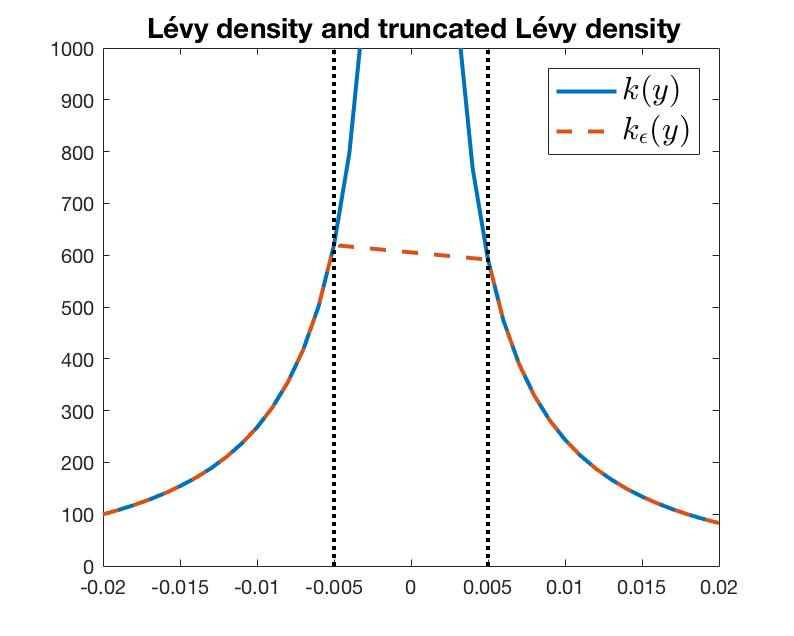
\includegraphics[scale=0.3]{gfx/Trunc_density}
	\caption{Pure jump L\'evy density (in blue) and its truncated density (in red) with $\epsilon = 0.005$.}
	\label{fig:FD:pj_density}
\end{figure}

We set now $\tilde{k}(y) = k(y) -k_\epsilon(y)$, which is non zero only for $|y|\leq\epsilon$, and split the integral terms as
$$\int_{-\infty}^\infty \left[V(x+y,\tau,A)-V(x,\tau,A)-\left(e^y-1\right)\frac{\partial V}{\partial x}(x,\tau,A)\right]k(y)dy =I_1+I_2,$$
with
\begin{align*}
I_1 &= \int_{-\infty}^{\infty}\left[V(x+y,\tau,A)-V(x,\tau,A)-\left(e^y-1\right)\frac{\partial V}{\partial x}(x,\tau,A)\right]k_\epsilon(y)dy\\
I_2 &= \int_{-\epsilon}^{\epsilon}\left[V(x+y,\tau,A)-V(x,\tau,A)-\left(e^y-1\right)\frac{\partial V}{\partial x}(x,\tau,A)\right]\tilde{k}(y)dy.
\end{align*}
The first term corresponds to the finite activity L\'evy process $X^\epsilon$ and can be treated as the previous case.

The second integral requires a bit more work. By summing and subtracting the term $y\frac{\partial V}{\partial x}$, we have
\begin{align*}
I_2 &= \int_{-\epsilon}^{\epsilon}\Bigg[\underbrace{V(x+y,\tau,A)-V(x,\tau,A)-y\frac{\partial V}{\partial x}(x,\tau,A)}_{\frac{y^2}{2}\frac{\partial^2V}{\partial x^2}+\mathcal{O}(y^3)}-\underbrace{\left(e^y-1-y\right)}_{\frac{y^2}{2}+\mathcal{O}(y^3)}\frac{\partial V}{\partial x}(x,\tau)\Bigg]\tilde{k}(y)dy\\
&=\left(\frac{\partial^2 V}{\partial x^2}-\frac{\partial V}{\partial x}\right)\frac{\sigma^2(\epsilon)}{2}+\int_{-\epsilon}^\epsilon \mathcal{O}(y^3)\tilde{k}(y)dy,
\end{align*}
with $$\sigma^2(\epsilon) = \int_{-\epsilon}^\epsilon y^2\tilde{k}(y)dy.$$

Therefore, we can treat the infinite activity case with a finite activity process $X^\epsilon$ characterized by the L\'evy triplet $(\gamma^\ast,\sigma(\epsilon),k_\epsilon(y))$. Hence, up to $\mathcal{O}(\epsilon^3)$ terms, the option price $V(x,t)$ satisfies the modified PIDE

\begin{align*}\frac{\partial V}{\partial \tau}-\frac{1}{2}\sigma^2(\epsilon)\frac{\partial^2V}{\partial x^2}&-\left(r_d-r_f-\frac{1}{2}\sigma^2(\epsilon) -c(\epsilon)\right)\frac{\partial V}{\partial x}+(r_d +\lambda(\epsilon))V \\
&-\int_{-\infty}^\infty V(x+y,\tau,A)k_\epsilon(y) dy = 0,
\end{align*}
with
\begin{align*}
\lambda(\epsilon) &\equiv \int_{-\infty}^\infty k_\epsilon(y)dy,\\
c(\epsilon) &\equiv \int_{-\infty}^\infty \left(y^2-1\right)k_\epsilon(y)dy,\\
\sigma^2(\epsilon) &\equiv \int_{-\infty}^\infty y^2 k_\epsilon(y)dy.
\end{align*}

For more details about the consistency, stability and convergence of finite difference scheme for exponential L\'evy models, please see in the main reference of this section, \citep{CV05}.

\section{The Convolution Method}
\label{sec:methods:conv}
The idea of this method is to replace the finite difference scheme by the convolution method proposed by \citeauthor{Lor+08} \citeyearpar{Lor+08} \cite{Lor+08}, based on the \textit{Fast Fourier Transform} (FFT), is that we don't need to discretize time between fixing dates. Thus, the total computational cost of the method is reduced to $\mathcal{O}(N_\text{fix-dates} N_a M \log(M))$, where $M$ and $N_a$ are respectively the number of grid points used to discretize the stock price $S$ and the accumulated amount variable $A$. 

\subsection{Description of the method}
Consider $V(S(t_n),t_n,A)$ the value of our FX-TARN at the $n$\textsuperscript{th} fixing date. Therefore, we can write, under risk-neutral measure $\mathbb{Q}$,
\begin{align*}
V(S(t_n),t_n,A) &= \mathbb{E}^\mathbb{Q}\left[e^{-r\Delta_t}V(S(t_{n+1}),t_{n+1},A|S(t_n)\right]\\
&=e^{-r\Delta_t}\int_{-\infty}^\infty V(y,t_{n+1},A)f(y|S(t_n))dy,
\end{align*}
where $f(y|S(t_n))$ represents the transition density from $S(t_n)$ at $t_n$ to $y$ at $t_{n+1}$. Since we use exponential L\'evy processes to characterize the stock price $S(t_n) = e^{X(t_n)}$, the stock price process has independent increments and we can write
$$f(y|x) = f(y-x),$$
where $x = \log(S(t_n))$ and $y = \log(S(t_{n+1}))$.

By changing variables $z = y-x$, the value $V$ can be expressed as
\begin{equation}\label{conv}
V(x,t_n,A) = e^{-r\Delta_t}\int_{-\infty}^\infty V(x+z,t_{n+1},A)f(z)dz,
\end{equation}
which is a cross-correlation of the option value at time $t_{n+1}$ and the density $f(z)$. We can equivalently see that as a convolution of $V(t_{n+1})$ and the conjugate of $f(z)$.

Let us now define the Fourier transform.

\begin{defn}[Fourier Transform]\label{def:conv:FT}
Given $h\in L^1(\mathbb{R})$, i.e. $h$ is an integrable function, we denote by $\hat{h}$ the \textbf{Fourier transform} of $h$, defined by
$$\hat{h}(u) := \mathcal{F}\{h(t)\}(u) = \int_{-\infty}^\infty e^{iut} h(t) dt.$$
Moreover, if $\hat{h}\in L^1(\mathbb{R})$, the \textbf{inverse Fourier transform} is given by
$$h(t):=\mathcal{F}^{-1}\{\hat{h}(u)\}(t) = \frac{1}{2\pi}\int_{-\infty}^\infty e^{-iut}\hat{h}(u)du.$$
\end{defn}
Remark that since $f$ is the density function of the L\'evy process, the Fourier transform of $f$ correspond to the characteristic function $\Phi$ of the process $X = \{X_t,t\geq 0\}$.

Now if we damped the option value by a factor $\exp(\alpha x)$ and take the Fourier transform of equation \eqref{conv}, we get
\begin{align*}
e^{r\Delta_t}\mathcal{F}\{v(x,t_n,A)\}(u) &= \int_{-\infty}^\infty e^{iux} e^{\alpha x} \int_{-\infty}^\infty V(x+z,t_{n+1},A)dzdx \\
&= \int_{-\infty}^\infty e^{iu(x+z)}v(x+z,t_{n+1},A)e^{-iz(u-i\alpha)}f(z)dzdx,
\end{align*}
where $v(x,t,A) = e^{\alpha x}V(x,t,A)$ is the damped value option. Changing the order of integration, we obtain
\begin{align*}
e^{r\Delta_t}\mathcal{F}\{v(x,t_n,A)\}(u) &= \int_{-\infty}^\infty\int_{-\infty}^\infty e^{iuy}v(y,t_{n+1},A)dy~e^{-i(u-i\alpha) z}f(z)dz\\
&= \int_{-\infty}^\infty e^{iuy}v(y,t_{n+1},A)dy \int_{-\infty}^\infty e^{-i(u-i\alpha)z}f(z)dz \\
&= \mathcal{F}\{v(x,t_n,A)\}(u)\Phi(-(u-i\alpha)).
\end{align*}
The difference with the approach of \citeauthor{CM99} \citeyearpar{CM99} \cite{CM99} is that we take the transform with respect to the log-spot price instead the log-strike price.

\subsection{Implementation of the method}
The goal is now to compute the convolution 
\begin{equation}\label{eq18}
v(x) = \frac{1}{2\pi}\int_{-\infty}^\infty e^{-iux}\hat{v}(u)\Phi(-(u-i\alpha))du,
\end{equation}
where $\hat{v}(u)$ is the Fourier transform of $v$:
\begin{equation}\label{eq19}
\hat{v}(u) = \int_{-\infty}^\infty e^{iuy}v(y)dy.
\end{equation}
For notational convenience, we dropped the discounting factor out of the equation. We can approximate these both integrals by a discrete sum, that allows us to use FFT algorithm to compute them. Thus we have to construct uniform grids for $u,x$ and $y$:
\begin{align*}
u_j &= u_0 + j\Delta u,\\
x_j &= x_0 + j\Delta x,\\
y_j &= y_0 +j\Delta y,
\end{align*}
for $j = 0,\ldots,M-1$. We can take the same mesh size for the $x$- and $y$-grids, i.e. $\Delta x = \Delta y$. However, the Nyquist relation must be satisfied, i.e.
$$\Delta u \cdot \Delta y = \frac{2\pi}{M}.$$
The discretization of equations \eqref{eq18}, with a general Newton-C\^otes rule to approximate the equations \eqref{eq19}, gives us
$$v(x_p)\approx\frac{\Delta u \Delta y}{2\pi}\sum_{j=0}^{M-1}e^{-iu_jx_p}\Phi(-(u_j-i\alpha))\sum_{n=0}^{M-1}w_ne^{iu_jy_n}v(y_n),$$
for $p=0,\ldots,M-1$. 

Here, we will use the trapezoidal rule with the weights $w_n$:
$$w_0=w_{M-1} = \frac{1}{2},\qquad w_n = 1, \quad\text{for }n=1,\ldots,M-2.$$

Including the grids discretization in our approximation, we have
$$v(x_p) \approx\frac{e^{-iu_0(x_0+p\Delta y)}}{2\pi}\Delta u\sum_{j=0}^{M-1}e^{-ijp2\pi/M}e^{ij(y_0-x_0)\Delta u}\Phi(-(u_j-i\alpha))\hat{v}(u_j), $$
where the Fourier transform of $v$ is approximated by
$$\hat{v}(u_j) \approx e^{iu_0y_0}\Delta y \sum_{n=0}^{M-1}e^{ijn2\pi/M}e^{inu_0\Delta y}w_nv(y_n).$$

Let us now define the \textit{Discrete Fourier Transform} (DFT) and its inverse.
\begin{defn}[Discrete Fourier Transform]
The \textbf{Discrete Fourier Transform} (DFT) of $x$ is a vector $\hat{x}\in\mathbb{R}^M$ defined by
$$\mathcal{D}_j\{x_n\} := \hat{x}_j = \sum_{n=0}^{M-1}e^{ijn2\pi/M}x_n.$$

Its inverse is given by
$$\mathcal{D}_n^{-1}\{\hat{x}_j\} := x_n =\frac{1}{M} \sum_{j=0}^{M-1}e^{-ijn2\pi/N}x_j.$$

Be careful with the \textsc{Matlab} conventions where $\mathcal{D} \equiv\texttt{ifft}$ and $\mathcal{D}^{-1}\equiv\texttt{fft}$.
\end{defn}

If we set $u_0 = -M/2\Delta u$, we have that
\begin{align*}
e^{inu_0\Delta y}&=e^{in\pi}\\
&=\cos(n\pi)+i\sin(n\pi)\\
&=(-1)^n.
\end{align*}

Finally, we obtain the result
$$v(x_p) \approx e^{iu_0(y_0-x_0)}(-1)^p\mathcal{D}_p^{-1}\left\{e^{ij(y_0-x_0)\Delta u}\Phi(-(u_j-i\alpha))\mathcal{D}_j\left\{(-1)^nw_nv(y_n)\right\}\right\}.$$

Thus, we have just to undamped the quantity $v(x,t_n,A)$ and discount the result to get the value $V(x,t_n,A)$ of the financial product.

\section{Summary}
\label{sec:methods:summary}
To conclude this chapter, we can summarize the whole algorithm of the two last methods.
\begin{enumerate}
\item Apply the zero final condition at $T = t_N$ for all the $N_a$ solutions to equation \eqref{eq:PDE} corresponding to $A_j, 1\leq j\leq N_a$.
\item Apply the jump condition to obtain $A^+_j = A^+_j + \tilde{C}_n$, where $\tilde{C}_n$ is the positive gain on the fixing date $t_n$.
\item Perform the cubic spline interpolation from points $V(S_m,t_n,A_j), j = 1,\ldots,N_a,$ to new points $V(S_m,t_n,A^+_j)$ for each spot grid points $S_m$.

\item Add the total cash flow $C^\text{tot}_n$ respecting the knock-out condition imposed by the accumulated amount. This leads to the value $V(S_m,t_n^-,A_j)$ expressed by equation \eqref{eq:jump_cond}.

\item Perform the \textbf{finite difference} or the \textbf{convolution method} for each $N_a$ solutions $V(S_m,t_n^-,A_j),j=1,\ldots,N_a,$ corresponding to the $N_a$ grid points in the auxiliary variable $A$. This gives us the value $V(S_m,t_{n-1},A_j)$ for $m=1,\ldots,M$.

\item Repeat steps 2 to 5 until $n = 0$ to get the today's value $V(S_m,t_0,A_j)$. Note that only the value for $A_0 = 0$ interests us, since at the beginning no amount is accumulated. Then the fair price of the FX-TARN is given by $V(S,t_0,0)$.
\end{enumerate}
%% !TEX root = ../thesis-example.tex
%
\chapter{Related Work}
\label{sec:related}

\cleanchapterquote{A picture is worth a thousand words. An interface is worth a thousand pictures.}{Ben Shneiderman}{(Professor for Computer Science)}

\Blindtext[2][1]

\section{Related Work Section 1}
\label{sec:related:sec1}

\Blindtext[2][2]

\section{Related Work Section 2}
\label{sec:related:sec2}

\Blindtext[3][2]

\section{Related Work Section 3}
\label{sec:related:sec3}

\Blindtext[4][2]

\section{Conclusion}
\label{sec:related:conclusion}

\Blindtext[2][1]
 % INCLUDE: related work
%% !TEX root = ../thesis-example.tex
%
\chapter{System}
\label{sec:system}

\cleanchapterquote{Innovation distinguishes between a leader and a follower.}{Steve Jobs}{(CEO Apple Inc.)}

\Blindtext[2][1]

\section{System Section 1}
\label{sec:system:sec1}

\Blindtext[1][2]

\begin{figure}[htb]
	
\includegraphics[width=\textwidth]{gfx/Clean-Thesis-Figure}
	\caption{Figure example: \textit{(a)} example part one, \textit{(c)} example part two; \textit{(c)} example part three}
	\label{fig:system:example1}
\end{figure}

\Blindtext[1][2]

\section{System Section 2}
\label{sec:system:sec2}

\Blindtext[1][2]

\begin{figure}[htb]
	
\includegraphics[width=\textwidth]{gfx/Clean-Thesis-Figure}
	\caption{Another Figure example: \textit{(a)} example part one, \textit{(c)} example part two; \textit{(c)} example part three}
	\label{fig:system:example2}
\end{figure}

\Blindtext[2][2]

\section{System Section 3}
\label{sec:system:sec3}

\Blindtext[4][2]

\section{Conclusion}
\label{sec:system:conclusion}

\Blindtext[2][1]
	% INCLUDE: system
%% !TEX root = ../thesis-example.tex
%
\chapter{Concepts: This text is here to test a very long title, to simulate the line break behavior, to show that an extremely long tilte also works}
\label{sec:concepts}

\cleanchapterquote{Users do not care about what is inside the box, as long as the box does what they need done.}{Jef Raskin}{about Human Computer Interfaces}

\Blindtext[2][1]

\section{Concepts Section 1}
\label{sec:concepts:sec1}

\Blindtext[2][2]

\section{Concepts Section 2}
\label{sec:concepts:sec2}

\Blindtext[3][2]

\section{Concepts Section 3}
\label{sec:concepts:sec3}

\Blindtext[4][2]

\section{Conclusion}
\label{sec:concepts:conclusion}

\Blindtext[2][1]
 % INCLUDE: concepts
%% !TEX root = ../thesis-example.tex
%
\chapter{Conclusion}
\label{sec:conclusion}

\Blindtext[2][1]

\section{System Section 1}
\label{sec:conclusion:sec1}

\Blindtext[2][2]

\section{System Section 2}
\label{sec:conclusion:sec2}

\Blindtext[3][2]

\section{Future Work}
\label{sec:conclusion:future}

\Blindtext[2][2]
 % INCLUDE: conclusion
\cleardoublepage

% --------------------------
% Back matter
% --------------------------
{%
\setstretch{1.1}
\renewcommand{\bibfont}{\normalfont\small}
\setlength{\biblabelsep}{0pt}
\setlength{\bibitemsep}{0.5\baselineskip plus 0.5\baselineskip}
\printbibliography%[nottype=online]
%\printbibliography[heading=subbibliography,title={Webseiten},type=online,prefixnumbers={@}]
}
\cleardoublepage

\listoffigures
\cleardoublepage

\listoftables
\cleardoublepage

% !TEX root = ../thesis-example.tex
%
\pagestyle{empty}
\hfill
\vfill
\pdfbookmark[0]{Colophon}{Colophon}
\section*{Colophon}

This thesis was typeset with \LaTeXe.
It uses the \textit{Clean Thesis} style developed by Ricardo Langner.
The design of the \textit{Clean Thesis} style is inspired by user guide documents from Apple Inc.

Download the \textit{Clean Thesis} style at \url{http://cleanthesis.der-ric.de/}.

\cleardoublepage

% !TEX root = ../thesis-example.tex
%
%************************************************
% Declaration
%************************************************
\pdfbookmark[0]{Declaration}{Declaration}
\chapter*{Declaration}
\label{sec:declaration}
\thispagestyle{empty}

You can put your declaration here, to declare that you have completed your work solely and only with the help of the references you mentioned.

\bigskip

\noindent\textit{\thesisUniversityCity, \thesisDate}

\smallskip

\begin{flushright}
	\begin{minipage}{5cm}
		\rule{\textwidth}{1pt}
		\centering\thesisName
	\end{minipage}
\end{flushright}

%*****************************************
%*****************************************

\clearpage
\newpage
\mbox{}

% **************************************************
% End of Document CONTENT
% **************************************************
\end{document}
